\section*{Введение}

В данной лабораторной работе рассматриваются линейные динамические системы второго порядка как в непрерывном, так и в дискретном времени. Динамические системы являются важным инструментом для моделирования различных физических, биологических и технических процессов.

\textbf{Цель работы:} изучение свойств устойчивости линейных динамических систем второго порядка, исследование влияния собственных чисел на характер движения системы и анализ физических интерпретаций.

\textbf{Задачи:}
\begin{enumerate}
    \item Создание и анализ непрерывных динамических систем с различными свойствами устойчивости
    \item Исследование дискретных динамических систем с заданными собственными числами
    \item Анализ осциллятора и его физических интерпретаций
\end{enumerate}

\section*{Задание 1. Непрерывные динамические системы}

\subsection*{Постановка задачи}

Рассматриваются непрерывные линейные динамические системы второго порядка вида:
\begin{equation}
\dot{x}(t) = Ax(t), \quad x(t) \in \mathbb{R}^2, \quad A \in \mathbb{R}^{2 \times 2}
\end{equation}

Заданы два неколлинеарных вектора $v_1 = (1, 2)$ и $v_2 = (2, -1)$, не лежащих на координатных осях. Требуется создать шесть различных систем с заданными свойствами.

\subsection*{Система 1: Асимптотически устойчива с инвариантными подпространствами}

\textbf{Требование:} Система асимптотически устойчива, при этом если $x(0) = v_1$, то $x(t) \in \text{Span}\{v_1\}$, а если $x(0) = v_2$, то $x(t) \in \text{Span}\{v_2\}$ при всех $t \geq 0$.

\textbf{Решение:} Создаем матрицу $A$ с собственными числами $\lambda_1 = -1$, $\lambda_2 = -2$ и собственными векторами $v_1$, $v_2$:
\begin{equation}
A = P \begin{pmatrix} -1 & 0 \\ 0 & -2 \end{pmatrix} P^{-1}
\end{equation}
где $P = [v_1, v_2]$.

\begin{figure}[H]
    \centering
    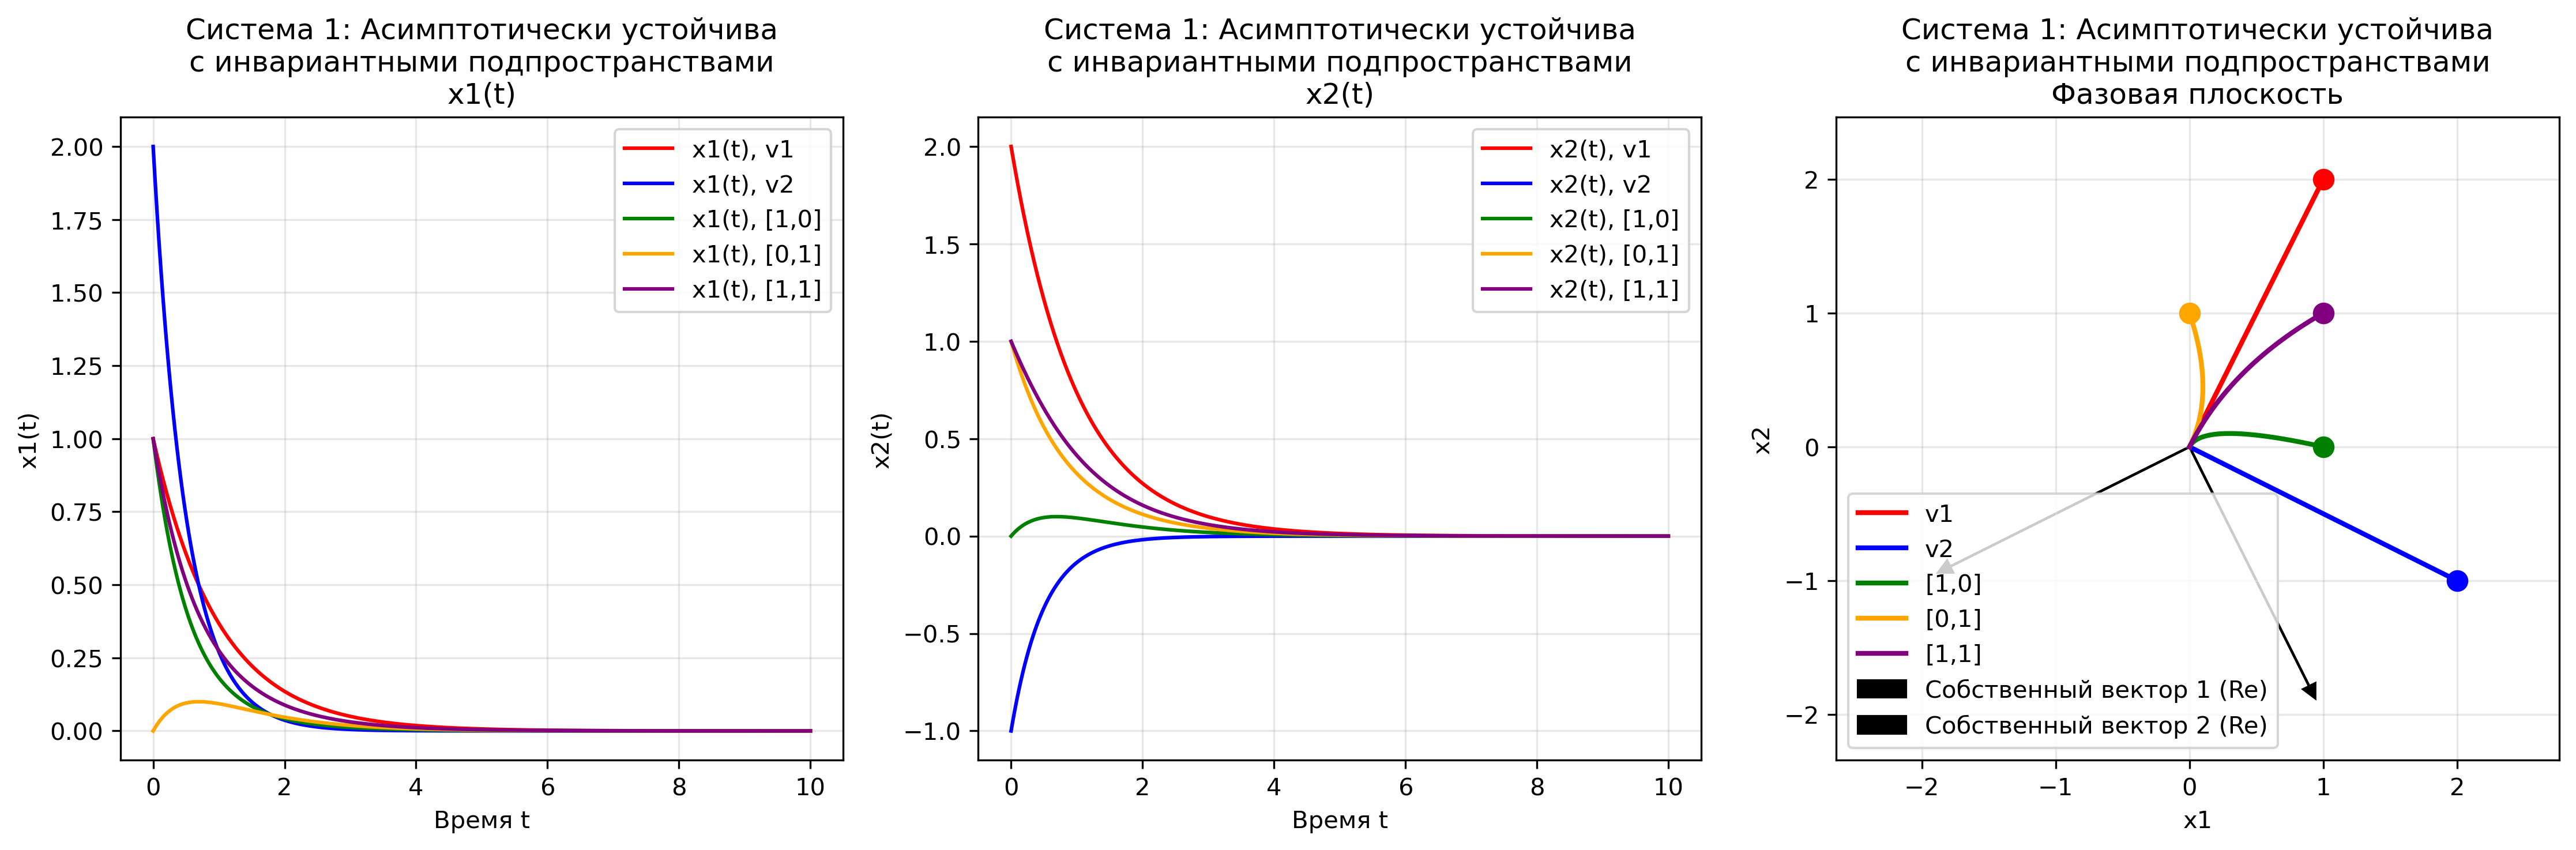
\includegraphics[width=0.9\textwidth]{images/task1/system1_asymptotically_stable.png}
    \caption{Система 1: Асимптотически устойчива с инвариантными подпространствами}
\end{figure}

\textbf{Анализ:}
\begin{itemize}
    \item Собственные числа: $\lambda_1 = -1$, $\lambda_2 = -2$ (оба отрицательные)
    \item Собственные векторы: $v_1 = (1, 2)$, $v_2 = (2, -1)$
    \item Система асимптотически устойчива, так как все собственные числа имеют отрицательные вещественные части
    \item Траектории, начинающиеся на собственных векторах, остаются в соответствующих подпространствах
\end{itemize}

\subsection*{Система 2: Неустойчива с дефектной матрицей}

\textbf{Требование:} Система неустойчива, при этом у матрицы $A$ не существует двух неколлинеарных собственных векторов.

\textbf{Решение:} Используем жорданову клетку с собственным числом $\lambda = 1$ кратности 2:
\begin{equation}
A = \begin{pmatrix} 1 & 1 \\ 0 & 1 \end{pmatrix}
\end{equation}

\begin{figure}[H]
    \centering
    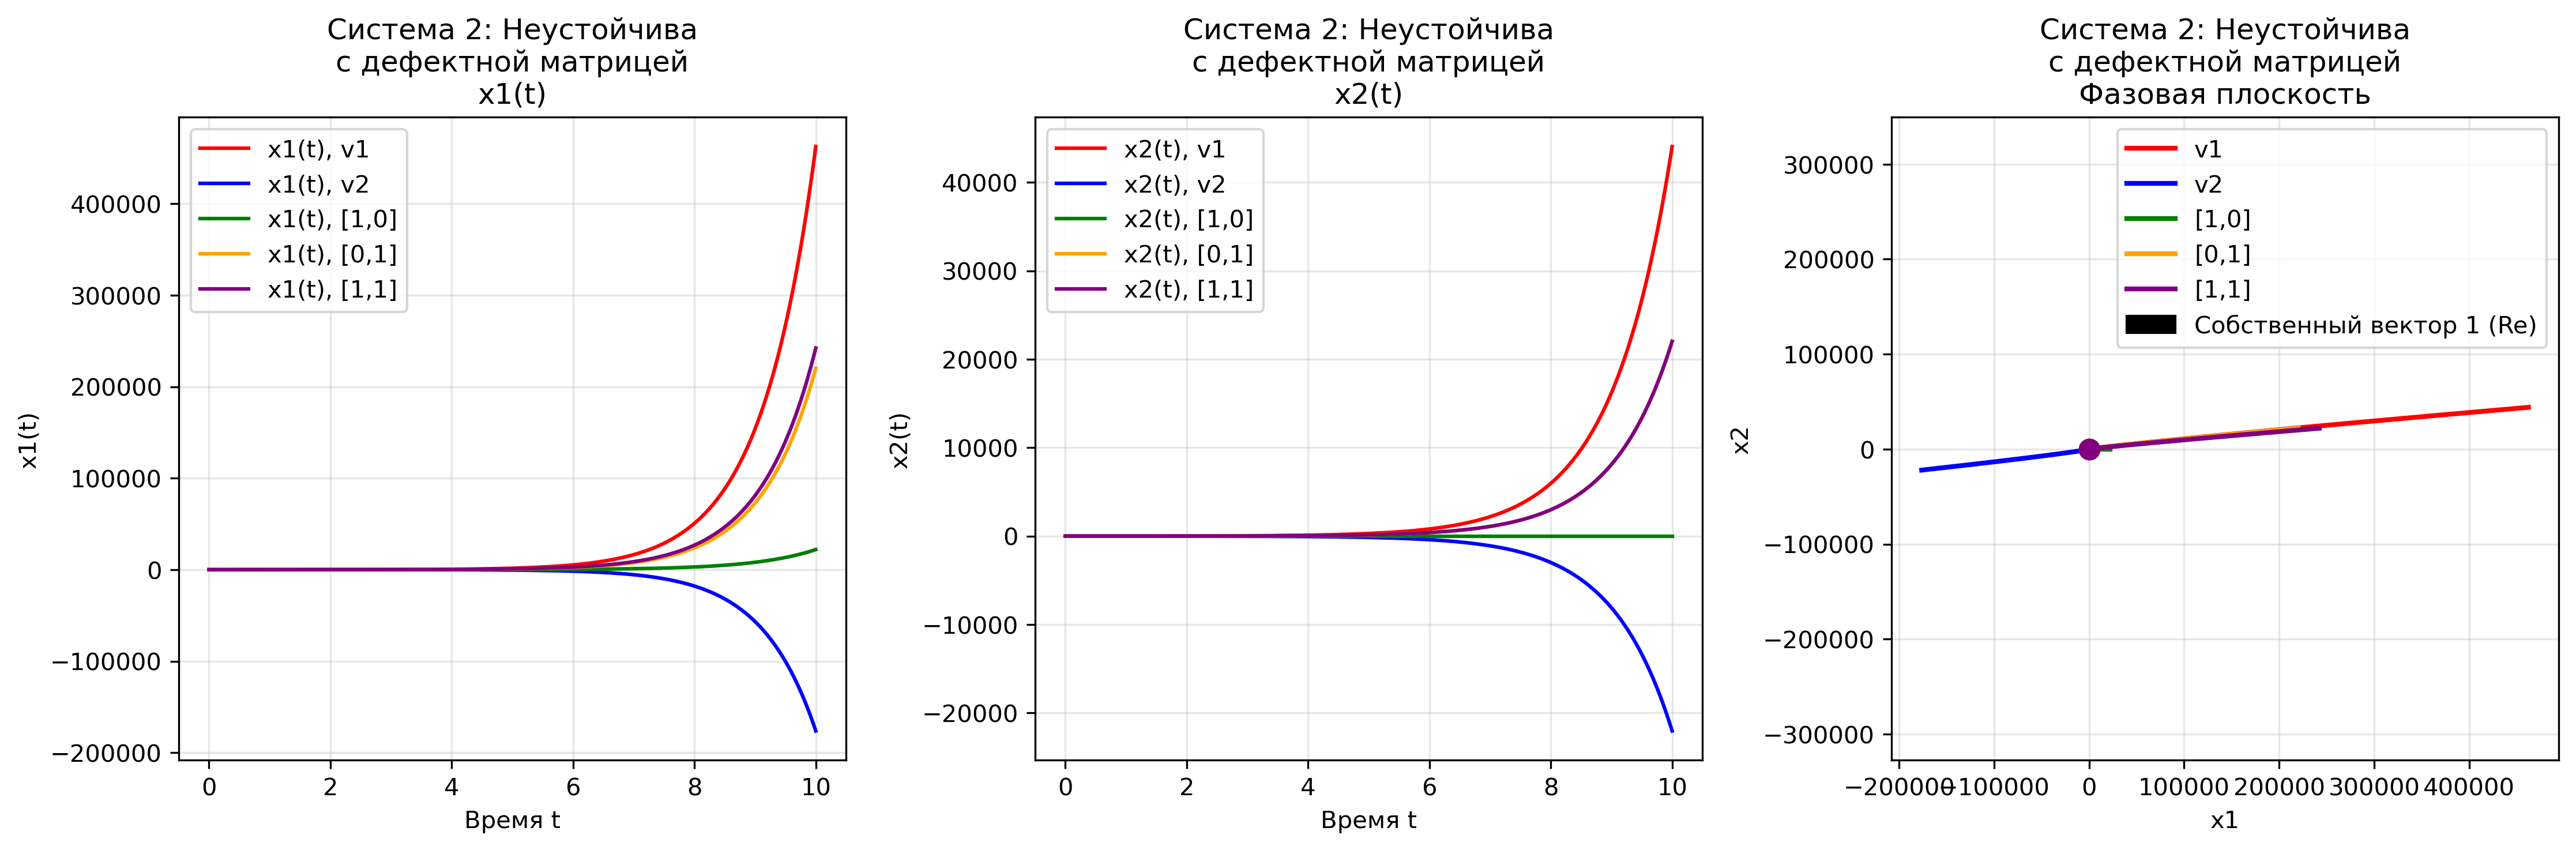
\includegraphics[width=0.9\textwidth]{images/task1/system2_unstable_defective.png}
    \caption{Система 2: Неустойчива с дефектной матрицей}
\end{figure}

\textbf{Анализ:}
\begin{itemize}
    \item Собственные числа: $\lambda_1 = \lambda_2 = 1$ (оба положительные)
    \item Матрица дефектная - имеет только один линейно независимый собственный вектор
    \item Система неустойчива, так как собственные числа положительные
    \item Траектории экспоненциально растут
\end{itemize}

\subsection*{Система 3: Неустойчива, но $v_1 \to 0$}

\textbf{Требование:} Система неустойчива, при этом если $x(0) = v_1$, то $\lim_{t \to \infty} x(t) = 0$.

\textbf{Решение:} Создаем матрицу с собственными числами $\lambda_1 = -1$, $\lambda_2 = 1$ и собственными векторами $v_1$, $v_2$:
\begin{equation}
A = P \begin{pmatrix} -1 & 0 \\ 0 & 1 \end{pmatrix} P^{-1}
\end{equation}

\begin{figure}[H]
    \centering
    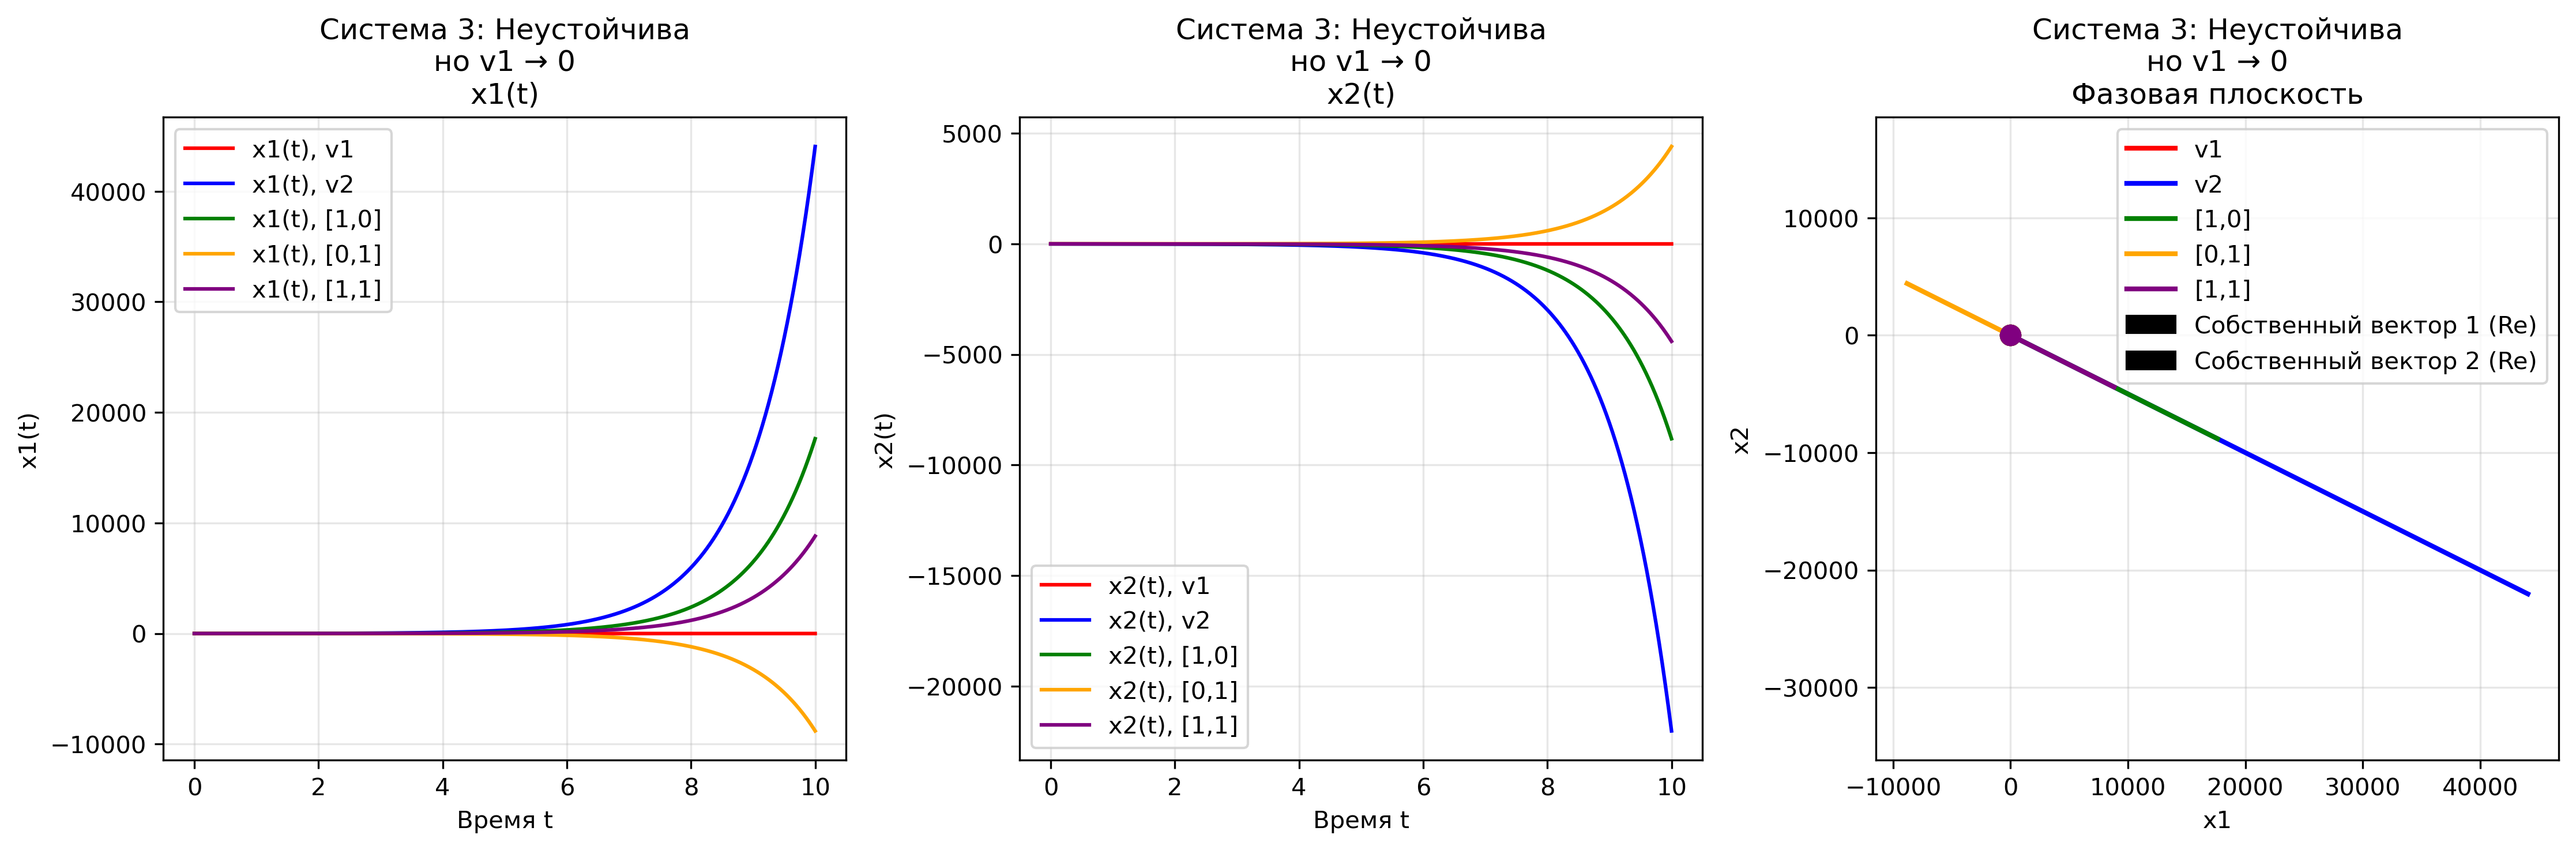
\includegraphics[width=0.9\textwidth]{images/task1/system3_unstable_v1_to_zero.png}
    \caption{Система 3: Неустойчива, но $v_1 \to 0$}
\end{figure}

\textbf{Анализ:}
\begin{itemize}
    \item Собственные числа: $\lambda_1 = -1$, $\lambda_2 = 1$ (одно отрицательное, одно положительное)
    \item Система неустойчива из-за положительного собственного числа
    \item Траектории, начинающиеся на $v_1$ (собственный вектор с отрицательным собственным числом), стремятся к нулю
    \item Траектории, начинающиеся на $v_2$ (собственный вектор с положительным собственным числом), растут
\end{itemize}

\subsection*{Система 4: Асимптотически устойчива с комплексными собственными векторами}

\textbf{Требование:} Система асимптотически устойчива, при этом матрица $A$ имеет комплексные собственные векторы вида $v_1 \pm v_2 i$.

\textbf{Решение:} Создаем матрицу с комплексными собственными числами $\lambda = -0.5 \pm 0.5i$:
\begin{equation}
A = \begin{pmatrix} -0.5 & -0.5 \\ 0.5 & -0.5 \end{pmatrix}
\end{equation}

\begin{figure}[H]
    \centering
    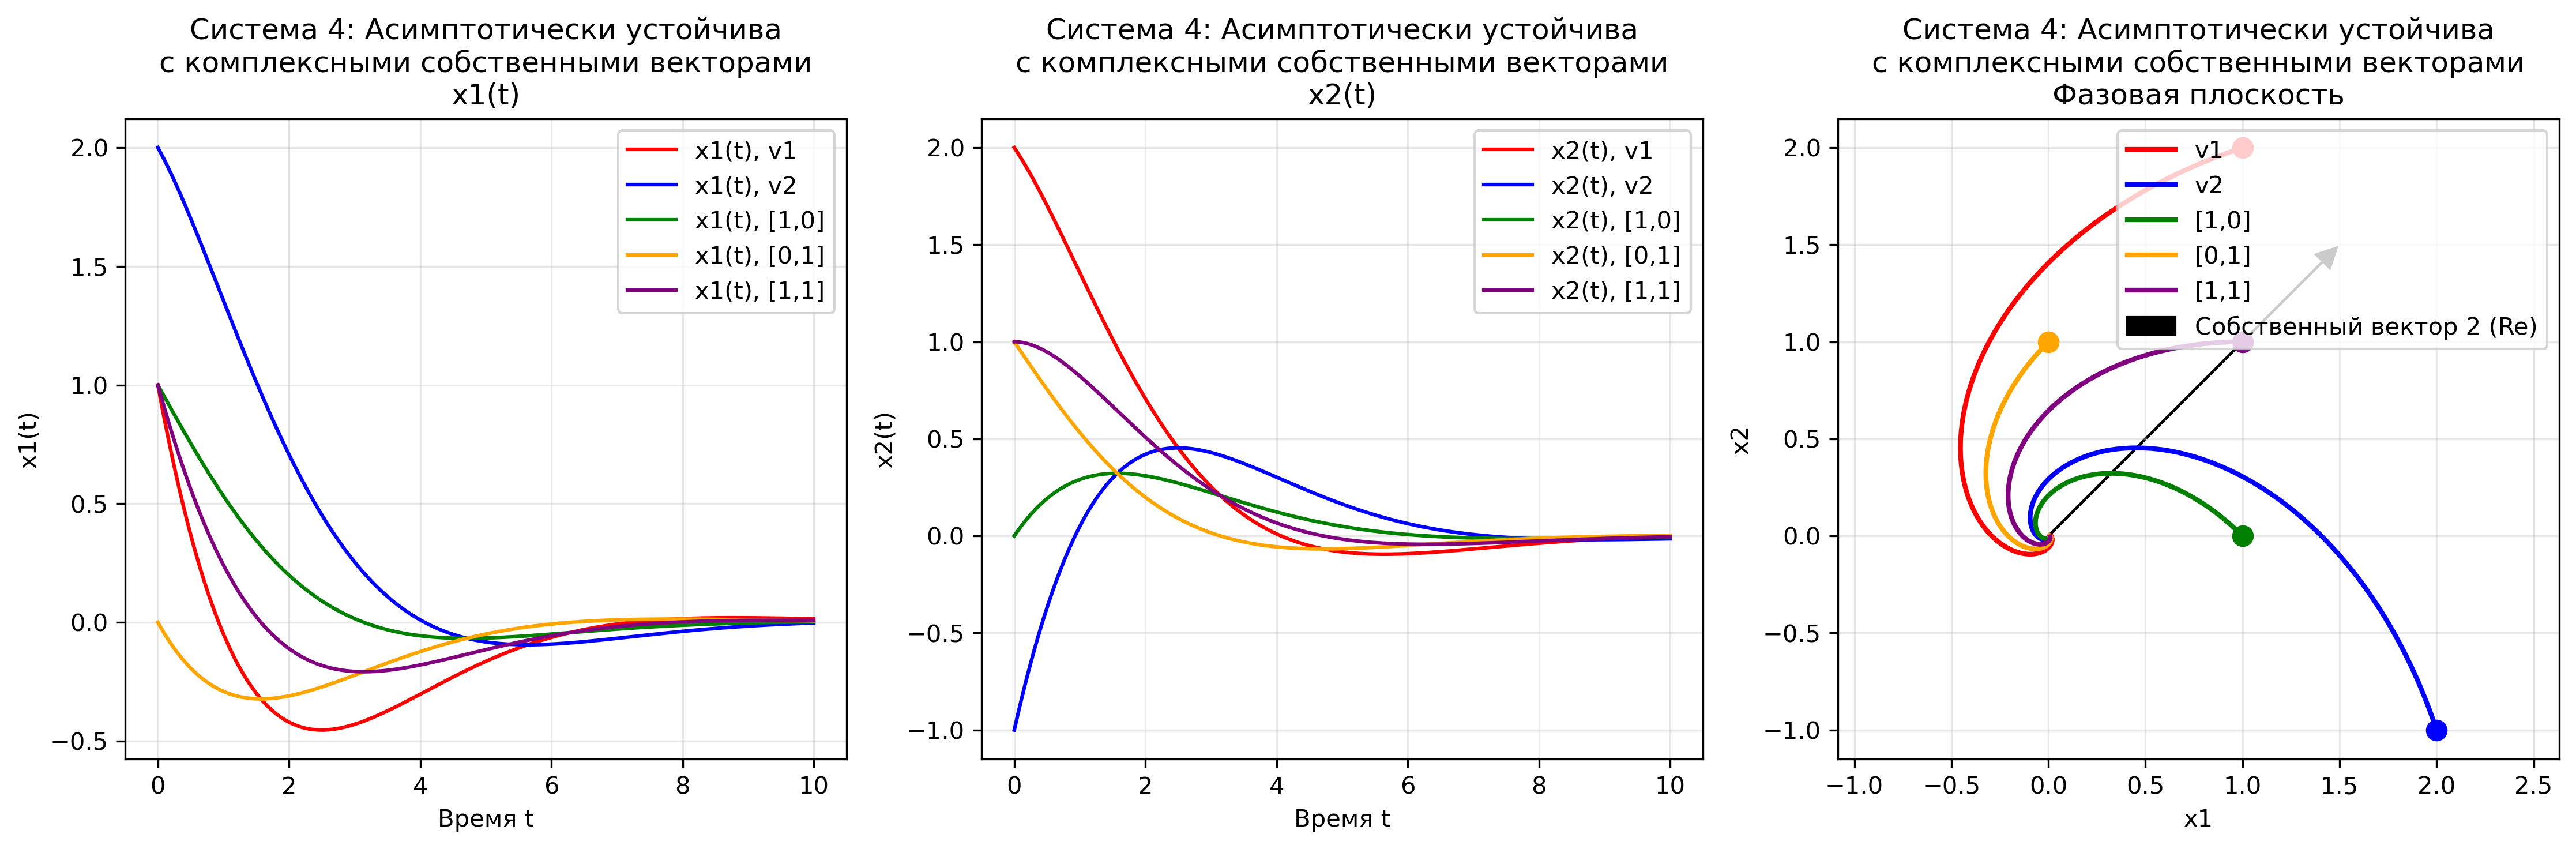
\includegraphics[width=0.9\textwidth]{images/task1/system4_asymptotically_stable_complex.png}
    \caption{Система 4: Асимптотически устойчива с комплексными собственными векторами}
\end{figure}

\textbf{Анализ:}
\begin{itemize}
    \item Собственные числа: $\lambda = -0.5 \pm 0.5i$ (отрицательные вещественные части)
    \item Собственные векторы: $v_1 \pm v_2 i$ (комплексные)
    \item Система асимптотически устойчива, так как вещественные части собственных чисел отрицательные
    \item Траектории затухают с колебаниями
\end{itemize}

\subsection*{Система 5: Неустойчива с комплексными собственными векторами}

\textbf{Требование:} Система неустойчива, при этом матрица $A$ имеет такие же собственные векторы, как в предыдущем пункте.

\textbf{Решение:} Создаем матрицу с комплексными собственными числами $\lambda = 0.5 \pm 0.5i$:
\begin{equation}
A = \begin{pmatrix} 0.5 & -0.5 \\ 0.5 & 0.5 \end{pmatrix}
\end{equation}

\begin{figure}[H]
    \centering
    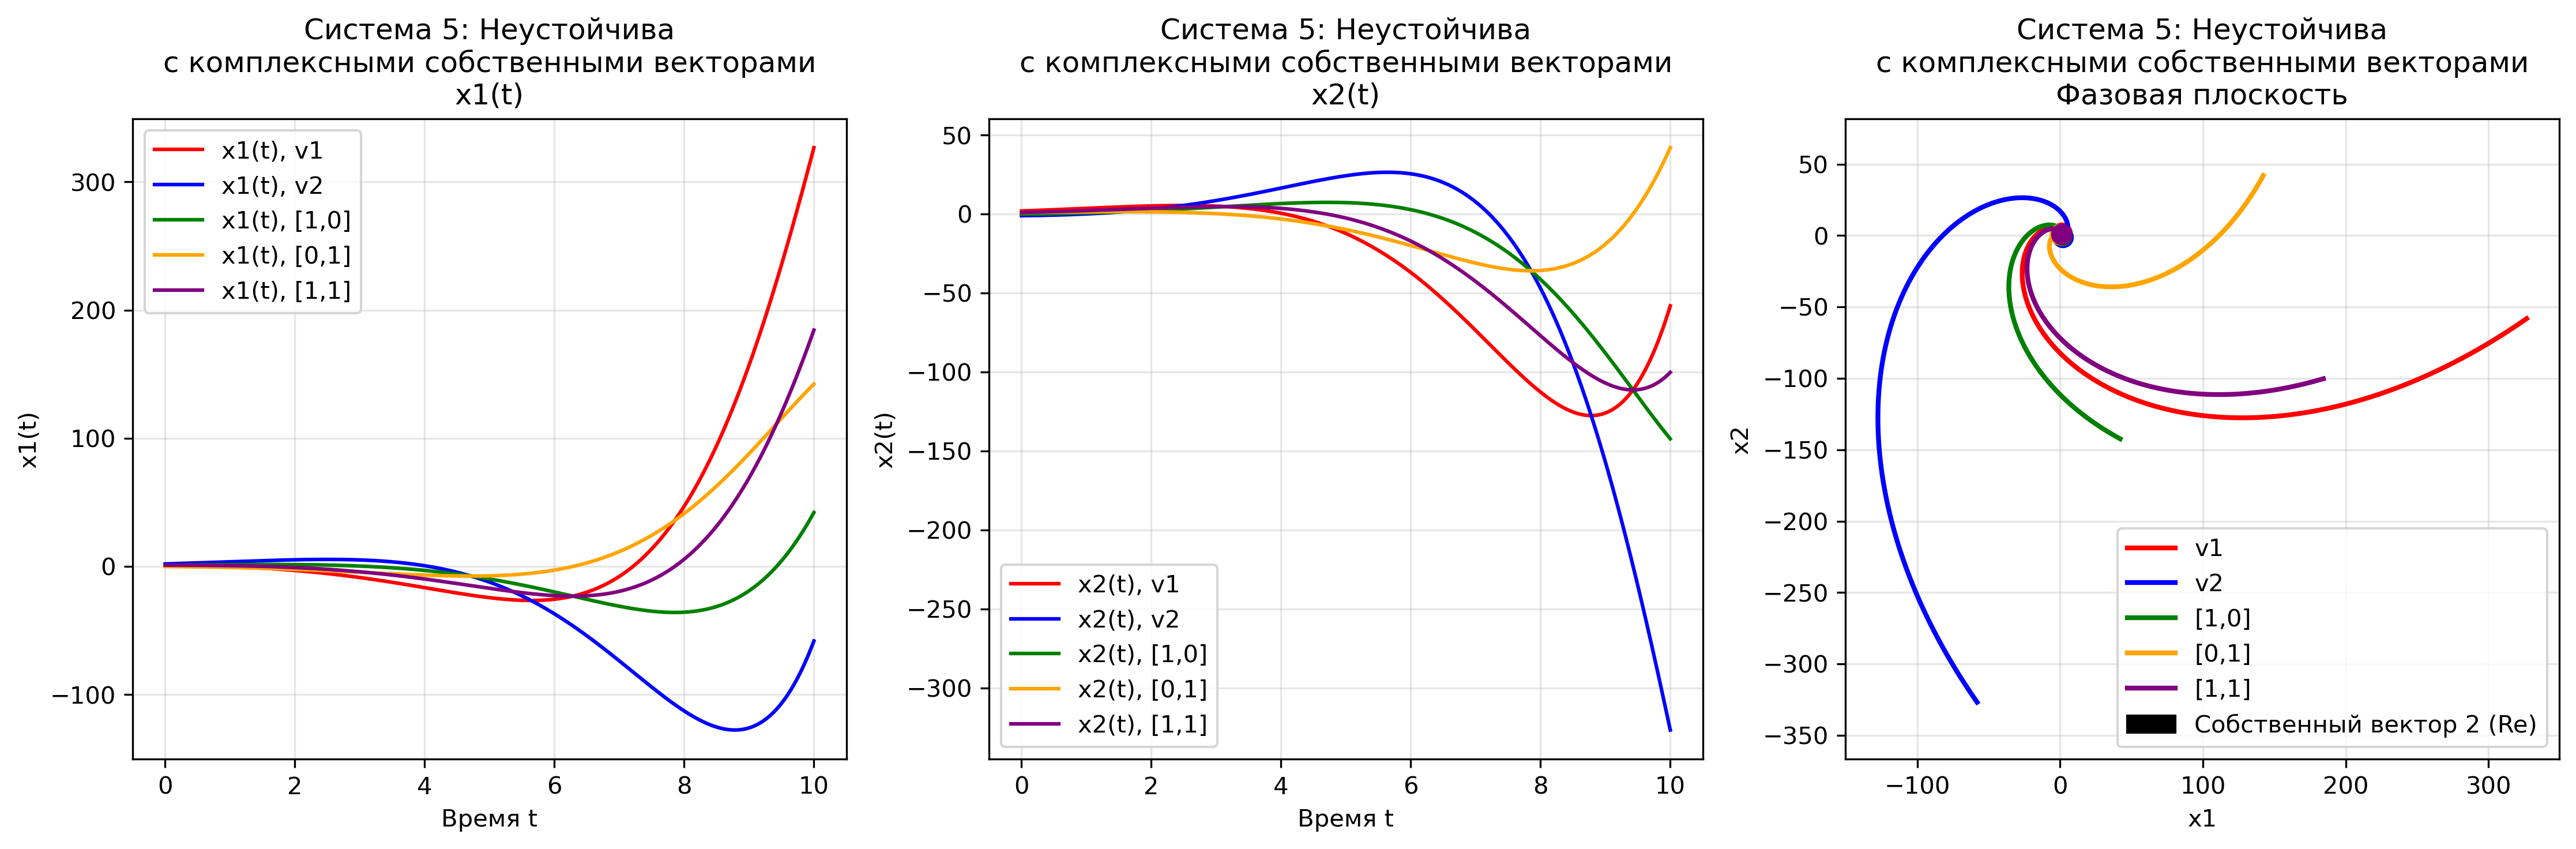
\includegraphics[width=0.9\textwidth]{images/task1/system5_unstable_complex.png}
    \caption{Система 5: Неустойчива с комплексными собственными векторами}
\end{figure}

\textbf{Анализ:}
\begin{itemize}
    \item Собственные числа: $\lambda = 0.5 \pm 0.5i$ (положительные вещественные части)
    \item Собственные векторы: $v_1 \pm v_2 i$ (комплексные)
    \item Система неустойчива, так как вещественные части собственных чисел положительные
    \item Траектории растут с колебаниями
\end{itemize}

\subsection*{Система 6: Нейтрально устойчива}

\textbf{Требование:} Система не является асимптотически устойчивой, но не является и неустойчивой, при этом матрица $A$ имеет собственные векторы такие же, как в пункте 4.

\textbf{Решение:} Создаем матрицу с чисто мнимыми собственными числами $\lambda = \pm i$:
\begin{equation}
A = \begin{pmatrix} 0 & -1 \\ 1 & 0 \end{pmatrix}
\end{equation}

\begin{figure}[H]
    \centering
    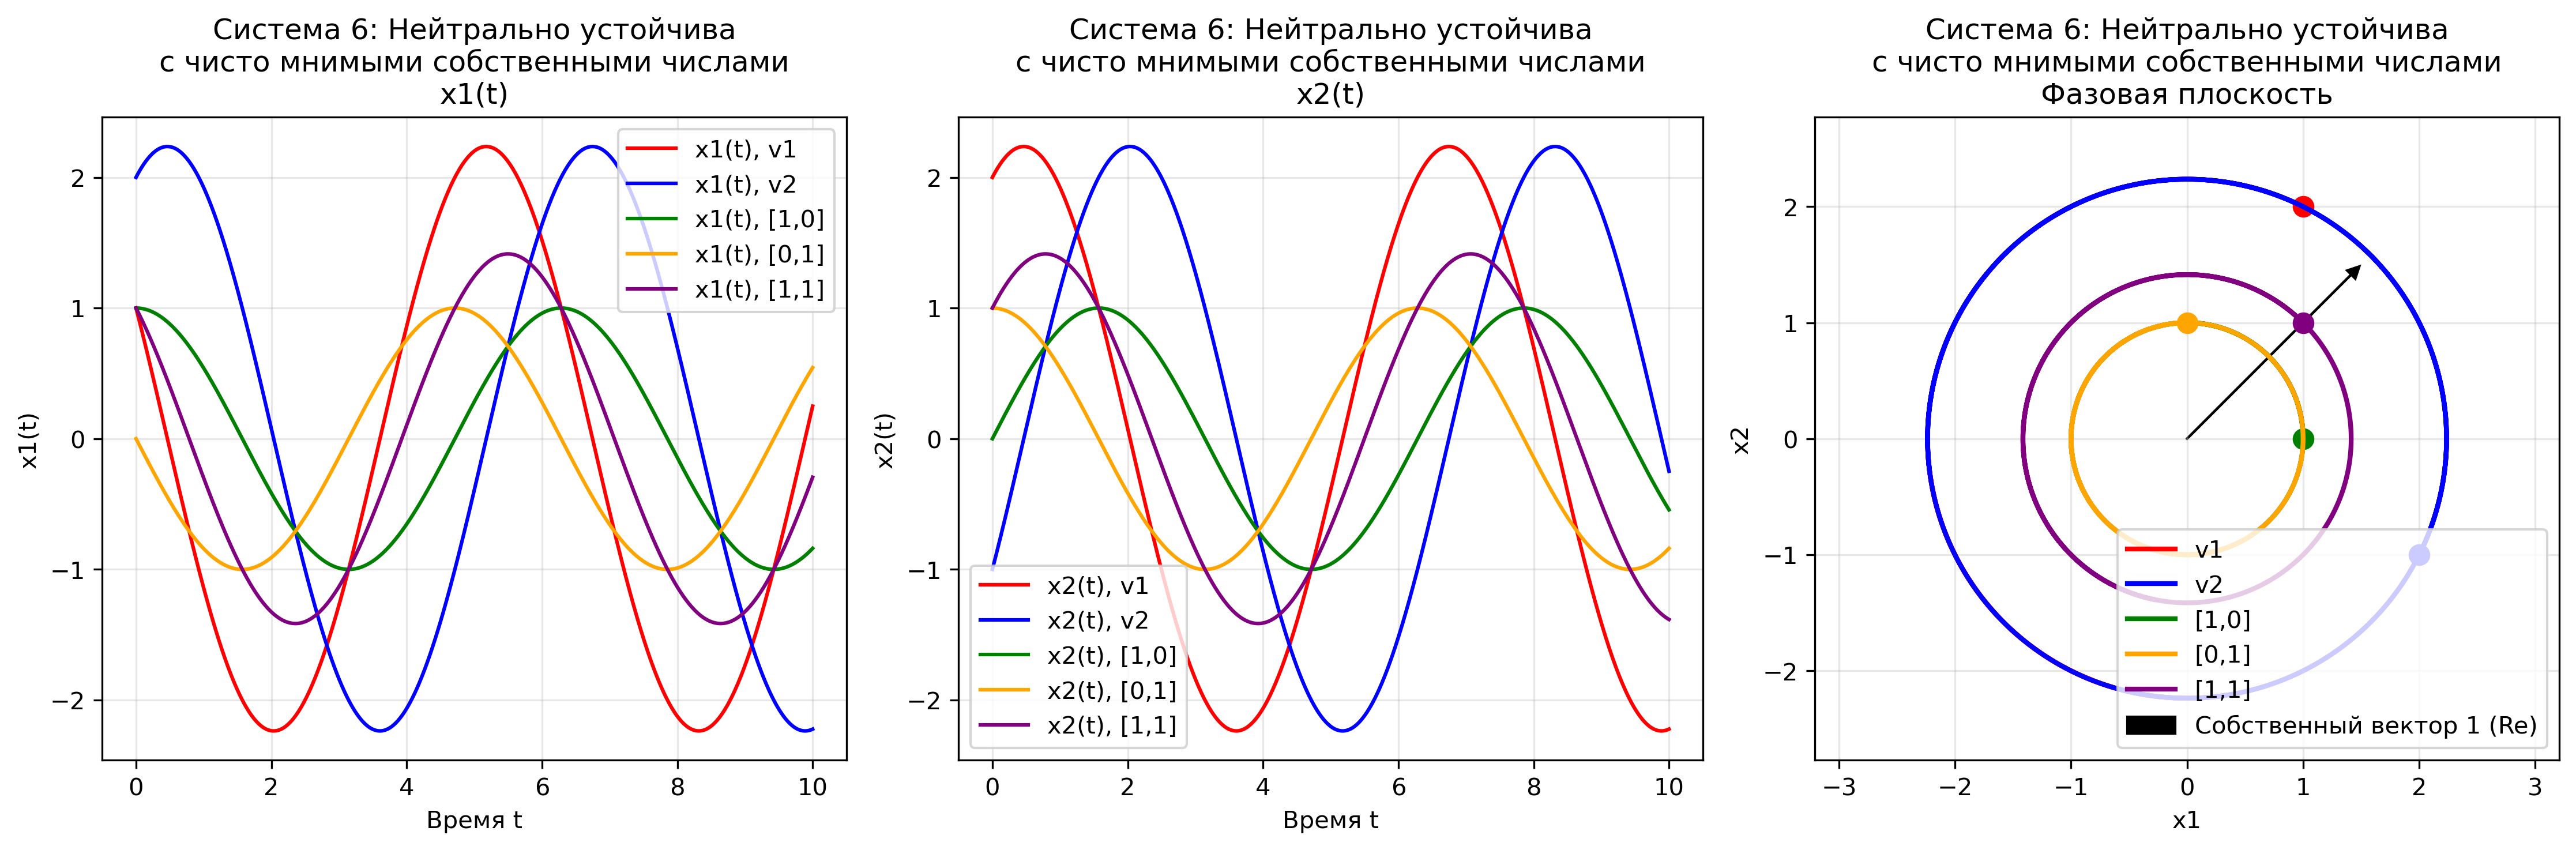
\includegraphics[width=0.9\textwidth]{images/task1/system6_neutrally_stable.png}
    \caption{Система 6: Нейтрально устойчива с чисто мнимыми собственными числами}
\end{figure}

\textbf{Анализ:}
\begin{itemize}
    \item Собственные числа: $\lambda = \pm i$ (чисто мнимые)
    \item Собственные векторы: $v_1 \pm v_2 i$ (комплексные)
    \item Система нейтрально устойчива, так как вещественные части собственных чисел равны нулю
    \item Траектории представляют собой замкнутые орбиты (периодические движения)
\end{itemize}

\section*{Задание 2. Дискретные динамические системы}

\subsection*{Постановка задачи}

Рассматриваются дискретные линейные динамические системы второго порядка вида:
\begin{equation}
x(k + 1) = Ax(k), \quad x(k) \in \mathbb{R}^2, \quad A \in \mathbb{R}^{2 \times 2}
\end{equation}

Требуется создать системы с заданными собственными числами и исследовать их поведение.

\subsection*{Системы с различными собственными числами}

Созданы следующие системы:

\begin{enumerate}
    \item $\lambda_{1,2} = -1$ - система с отрицательными собственными числами
    \item $\lambda_{1,2} = -\frac{1}{\sqrt{2}} \pm \frac{1}{\sqrt{2}}i$ - система с комплексными собственными числами, модуль которых равен 1
    \item $\lambda_{1,2} = \pm i$ - система с чисто мнимыми собственными числами
    \item $\lambda_{1,2} = \frac{1}{\sqrt{2}} \pm \frac{1}{\sqrt{2}}i$ - система с комплексными собственными числами, модуль которых равен 1
    \item $\lambda_{1,2} = 1$ - система с положительными собственными числами
\end{enumerate}

\begin{figure}[H]
    \centering
    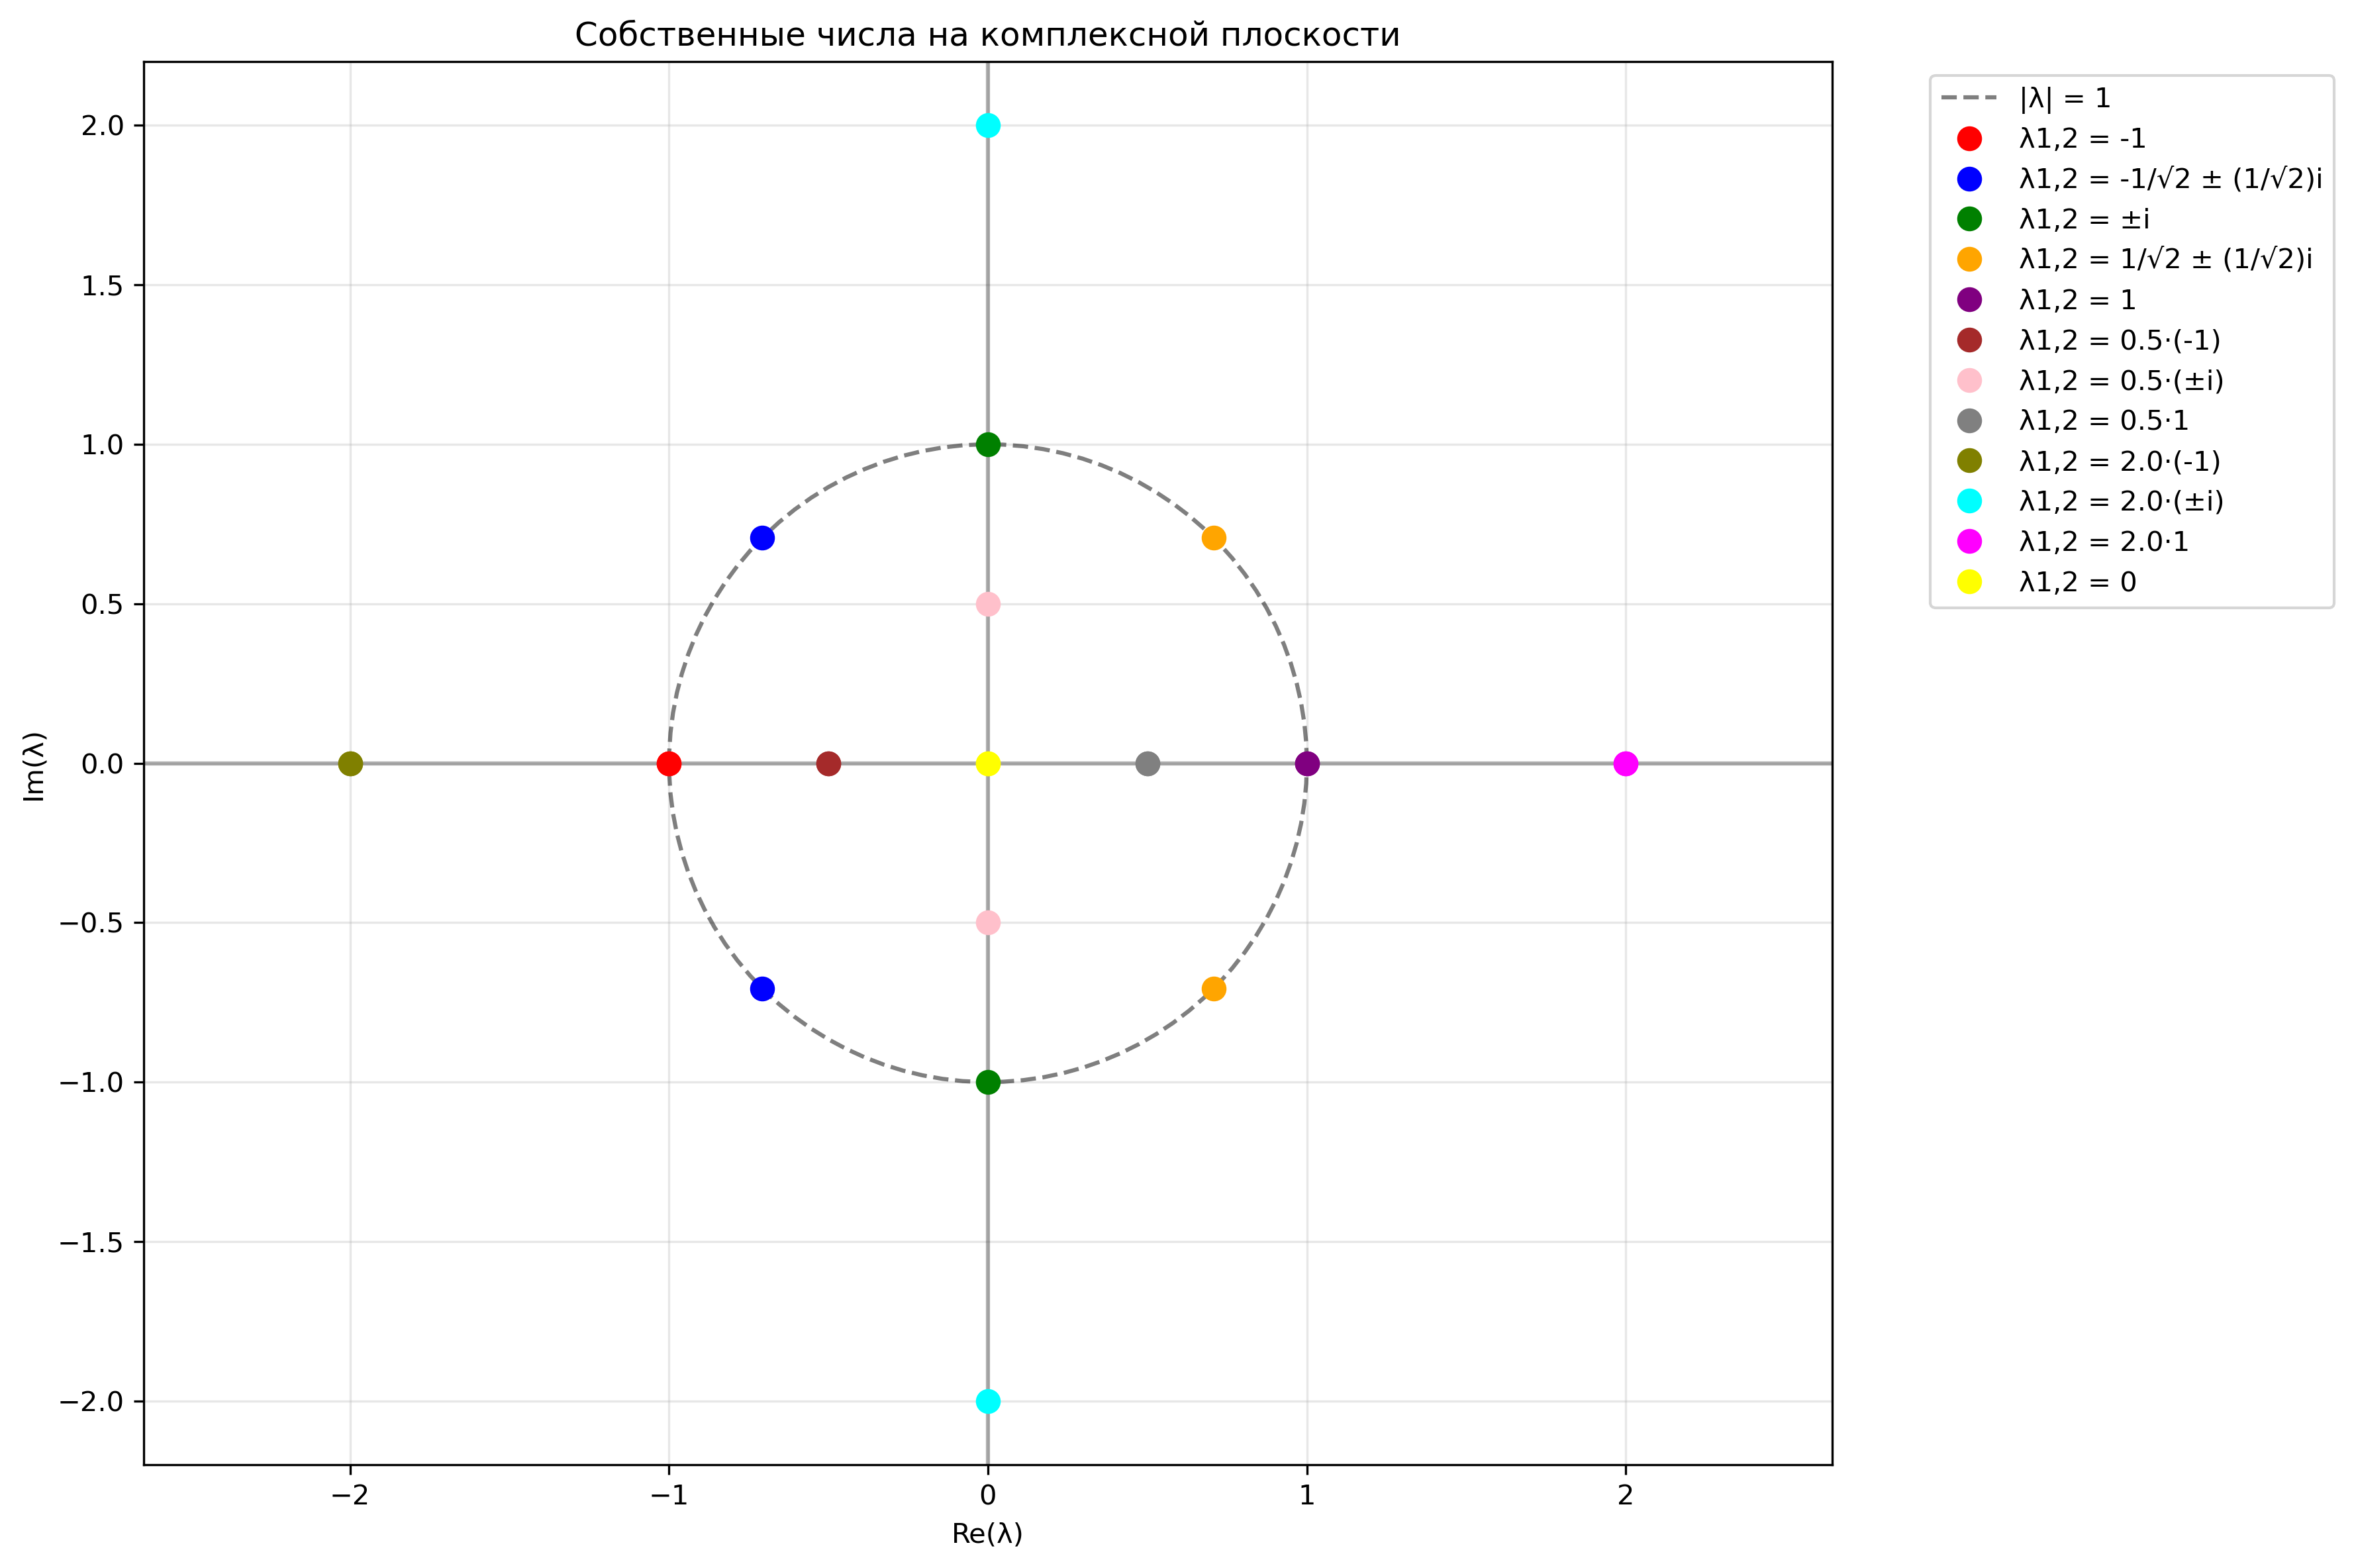
\includegraphics[width=0.9\textwidth]{images/task2/eigenvalues_complex_plane.png}
    \caption{Собственные числа всех систем на комплексной плоскости}
\end{figure}

\subsection*{Анализ влияния масштабирования}

Исследовано влияние масштабирования собственных чисел на поведение системы:

\begin{itemize}
    \item \textbf{Уменьшение масштаба} ($c = 0.5$): системы становятся более устойчивыми, траектории быстрее стремятся к нулю
    \item \textbf{Увеличение масштаба} ($d = 2.0$): системы становятся менее устойчивыми, траектории быстрее растут
\end{itemize}

\begin{figure}[H]
    \centering
    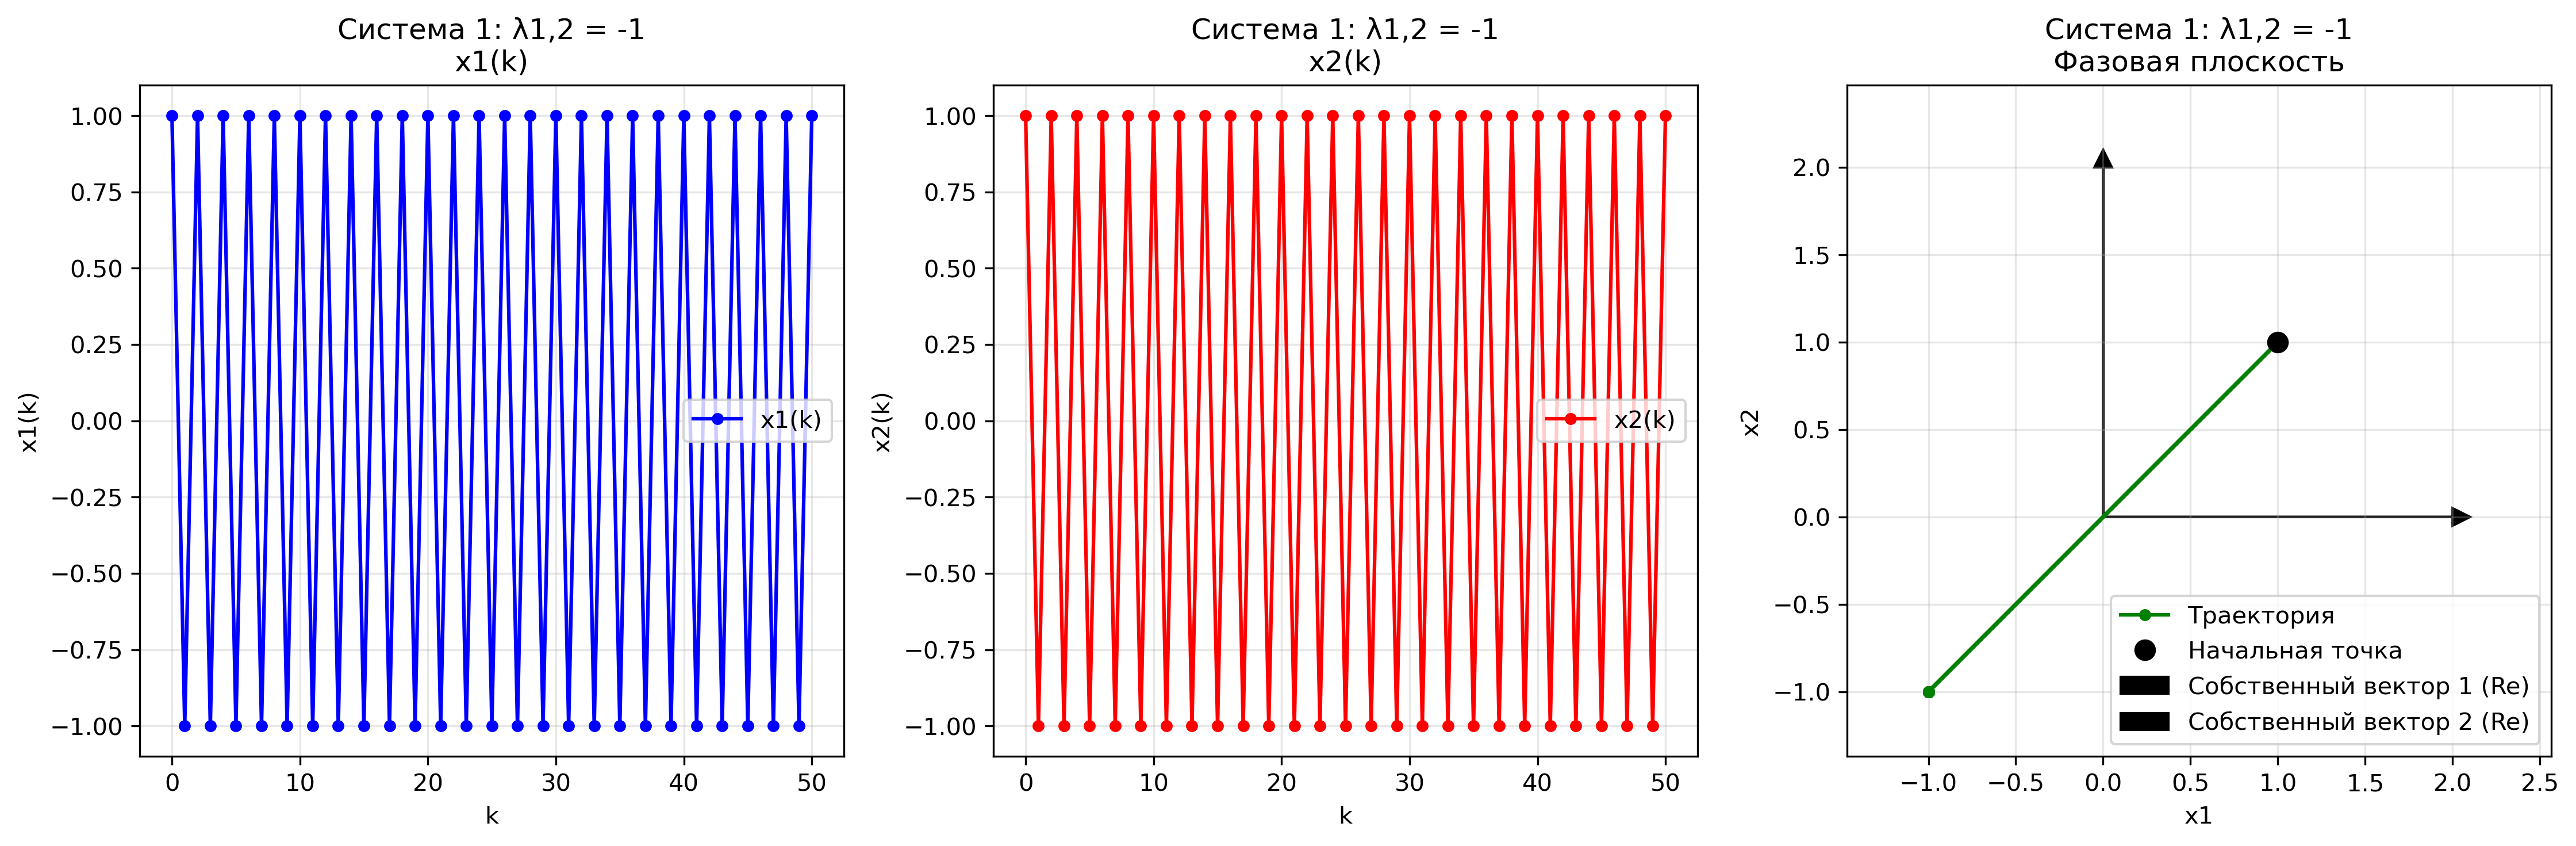
\includegraphics[width=0.9\textwidth]{images/task2/system1_lambda_minus1.png}
    \caption{Система 1: $\lambda_{1,2} = -1$}
\end{figure}

\begin{figure}[H]
    \centering
    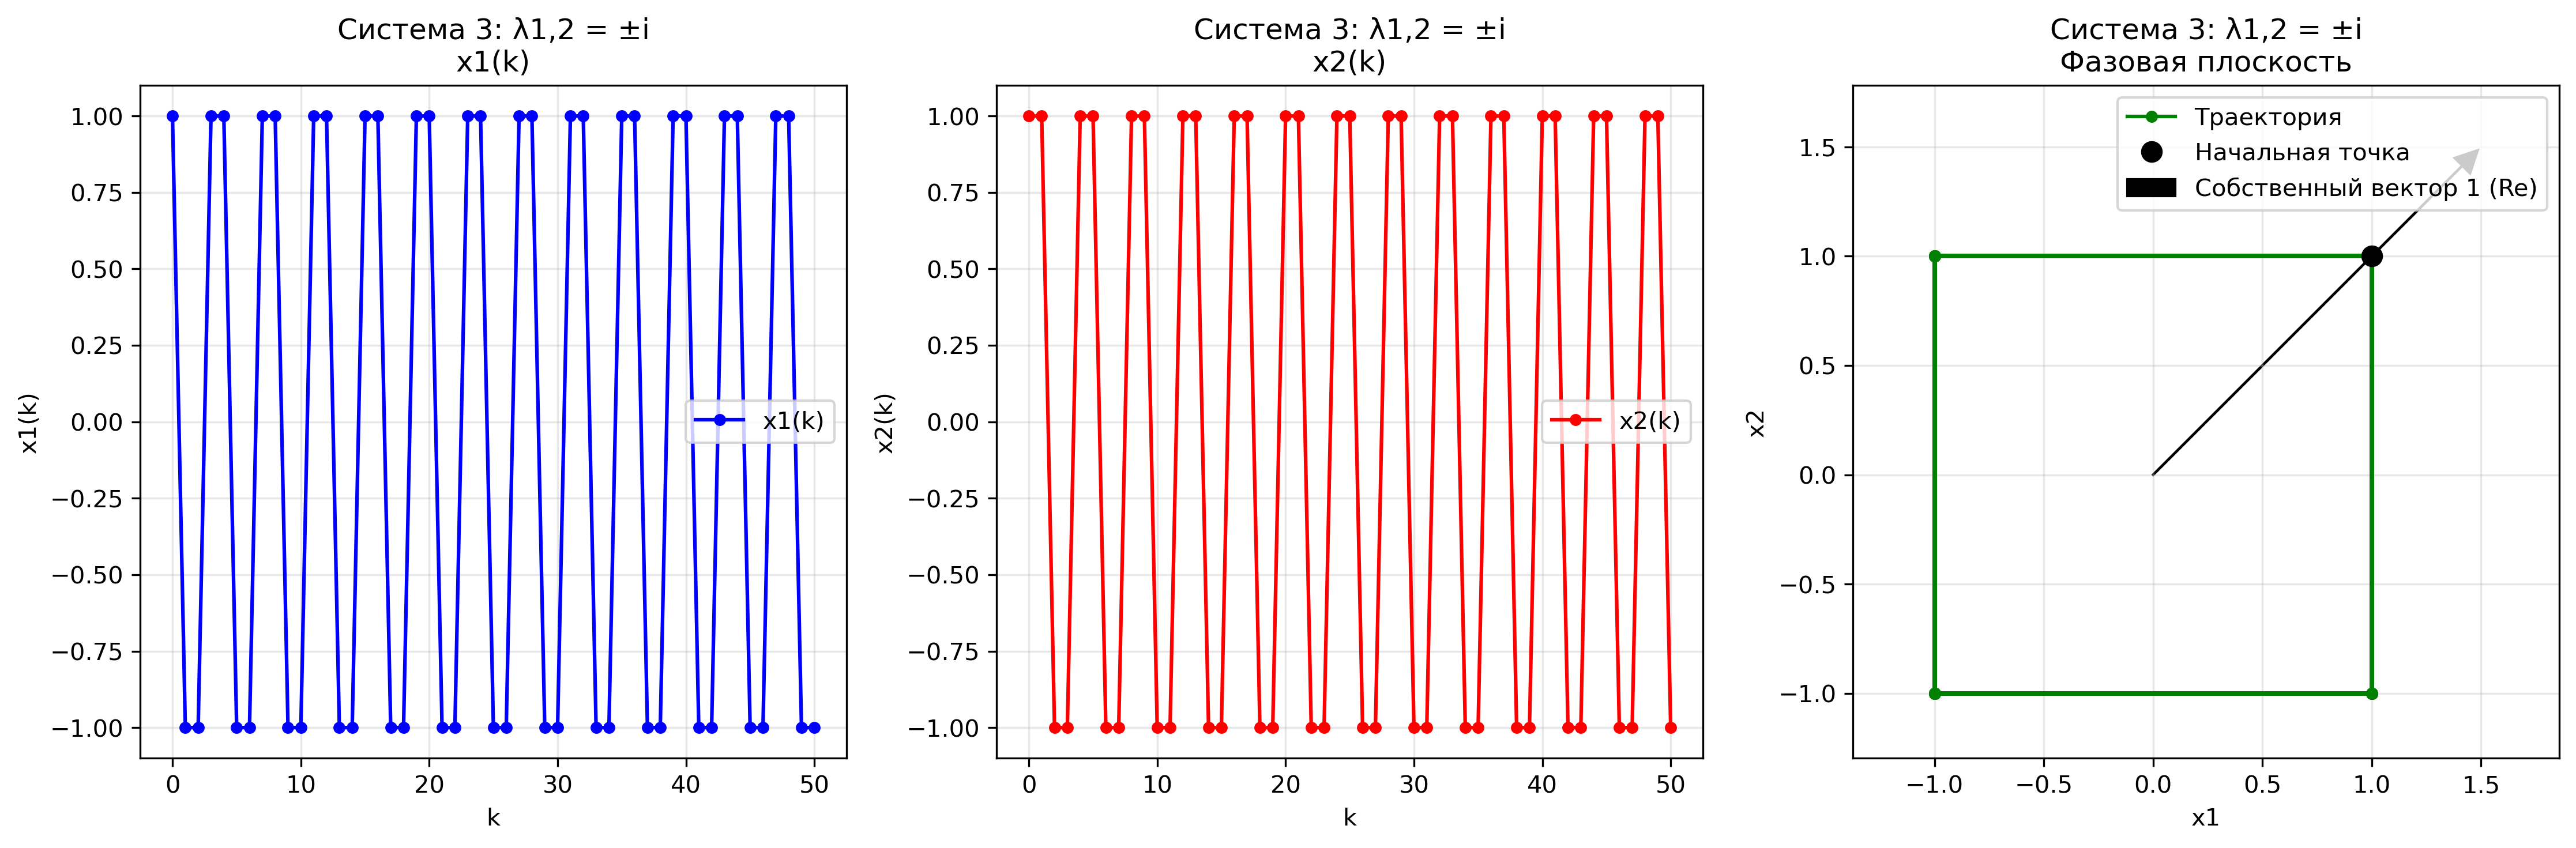
\includegraphics[width=0.9\textwidth]{images/task2/system3_lambda_pure_imaginary.png}
    \caption{Система 3: $\lambda_{1,2} = \pm i$}
\end{figure}

\begin{figure}[H]
    \centering
    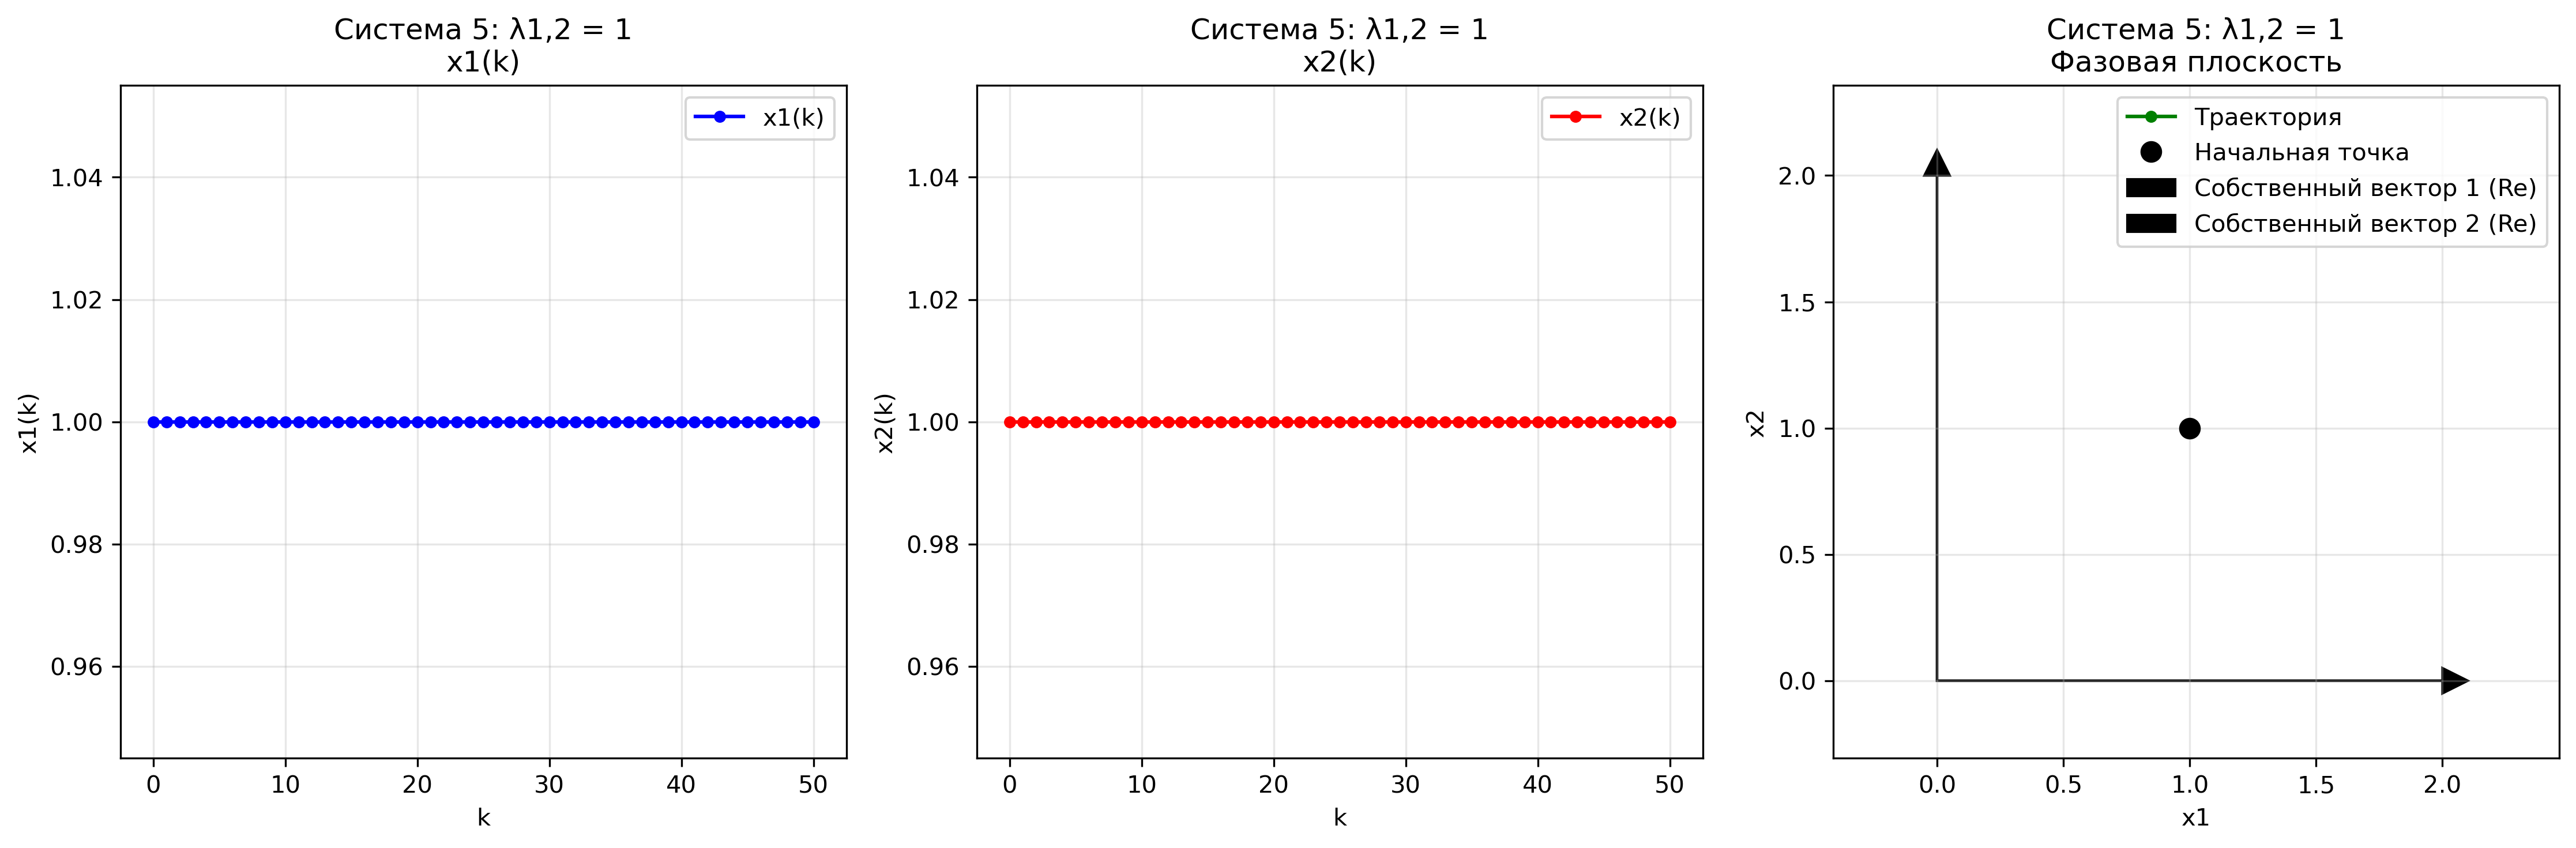
\includegraphics[width=0.9\textwidth]{images/task2/system5_lambda_plus1.png}
    \caption{Система 5: $\lambda_{1,2} = 1$}
\end{figure}

\subsection*{Закономерности поведения дискретных систем}

\begin{itemize}
    \item \textbf{$|\lambda| < 1$}: система асимптотически устойчива, траектории стремятся к нулю
    \item \textbf{$|\lambda| = 1$}: система нейтрально устойчива, траектории ограничены
    \item \textbf{$|\lambda| > 1$}: система неустойчива, траектории растут
    \item \textbf{Комплексные $\lambda$}: траектории имеют колебательный характер
    \item \textbf{Чисто мнимые $\lambda$}: траектории представляют собой замкнутые орбиты
\end{itemize}

\section*{Задание 3. Осциллятор}

\subsection*{Постановка задачи}

Рассматривается непрерывная система вида:
\begin{equation}
\begin{cases}
\dot{x}_1 = x_2 \\
\dot{x}_2 = ax_1 + bx_2
\end{cases}
\end{equation}

Требуется проанализировать устойчивость и характер движения при различных значениях параметров $a$ и $b$.

\subsection*{Случай 1: $a < 0$, $b = 0$ (Гармонический осциллятор)}

\textbf{Физическая интерпретация:} Гармонический осциллятор (пружина без трения)

\begin{itemize}
    \item $x_1$ - смещение от положения равновесия
    \item $x_2$ - скорость
    \item $a < 0$ - коэффициент упругости (отрицательный для возвращающей силы)
    \item $b = 0$ - отсутствие трения
\end{itemize}

\begin{figure}[H]
    \centering
    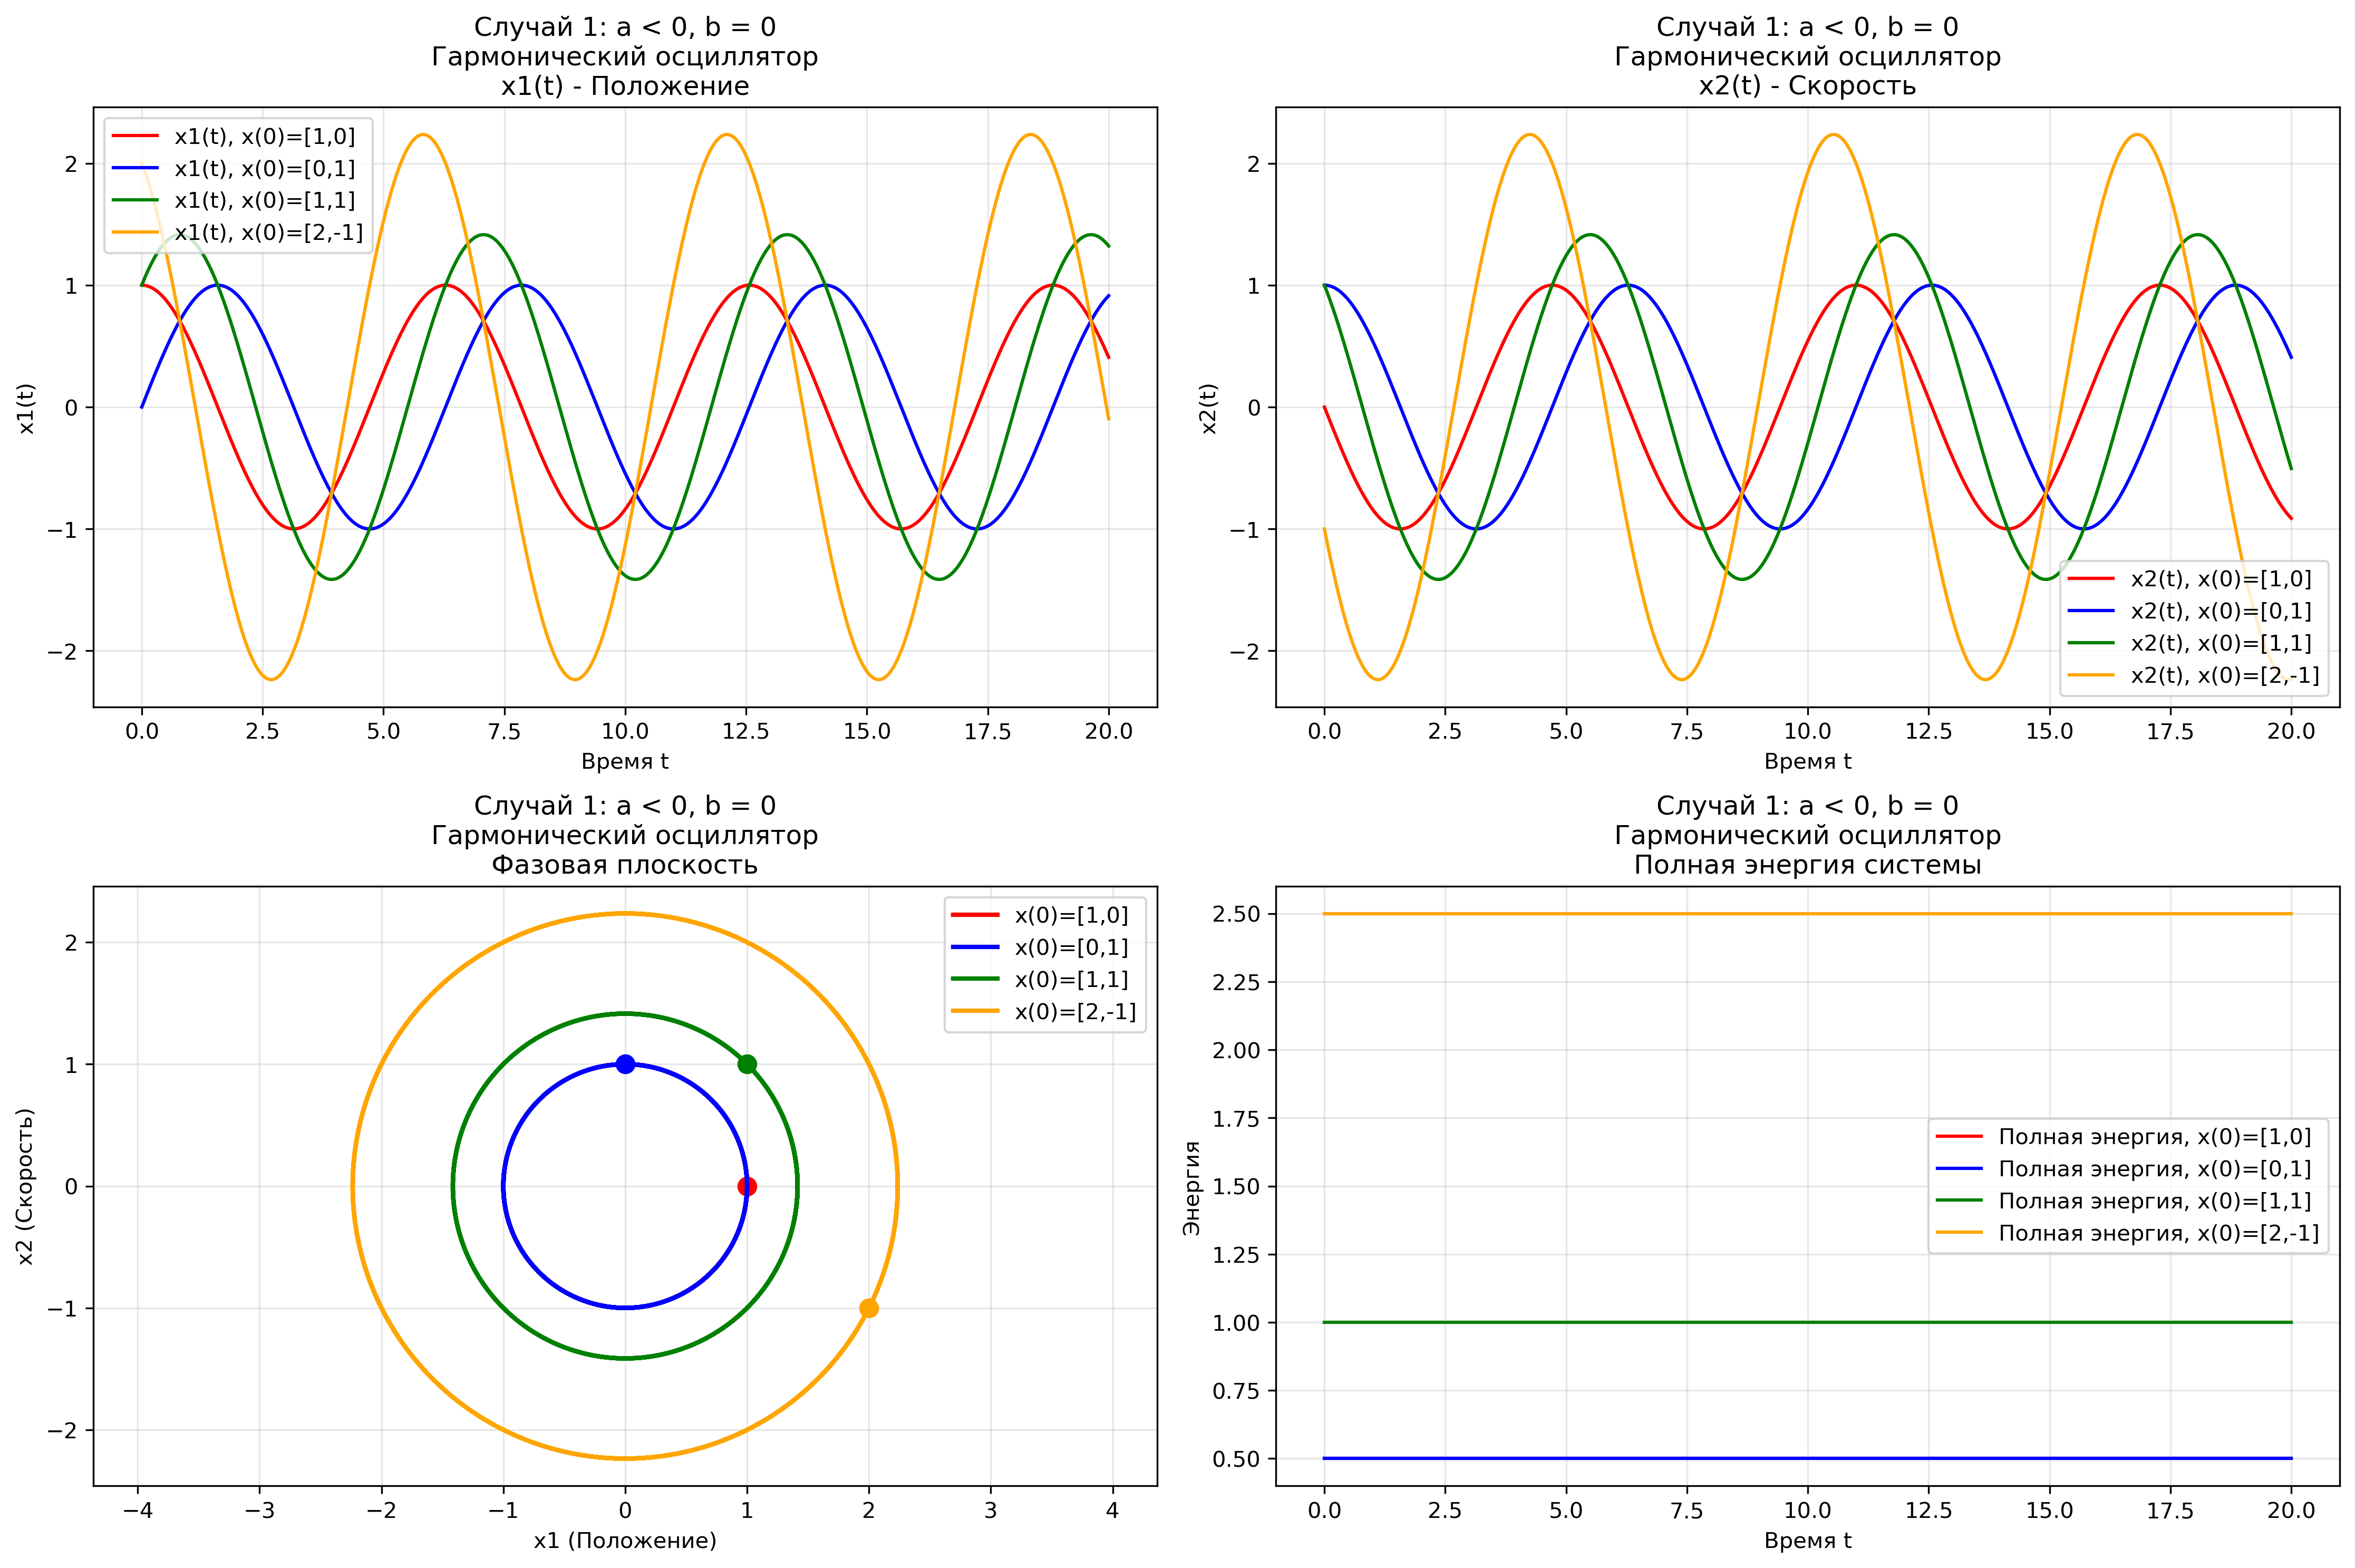
\includegraphics[width=0.9\textwidth]{images/task3/oscillator_case1_harmonic.png}
    \caption{Гармонический осциллятор: $a = -1$, $b = 0$}
\end{figure}

\textbf{Анализ:}
\begin{itemize}
    \item Собственные числа: $\lambda = \pm i$ (чисто мнимые)
    \item Тип устойчивости: Нейтрально устойчива
    \item Характер движения: Периодические колебания с постоянной амплитудой
    \item Энергия системы сохраняется
\end{itemize}

\subsection*{Случай 2: $a < 0$, $b < 0$ (Затухающий осциллятор)}

\textbf{Физическая интерпретация:} Затухающий осциллятор (пружина с трением)

\begin{itemize}
    \item $x_1$ - смещение от положения равновесия
    \item $x_2$ - скорость
    \item $a < 0$ - коэффициент упругости
    \item $b < 0$ - коэффициент трения (отрицательный для затухания)
\end{itemize}

\begin{figure}[H]
    \centering
    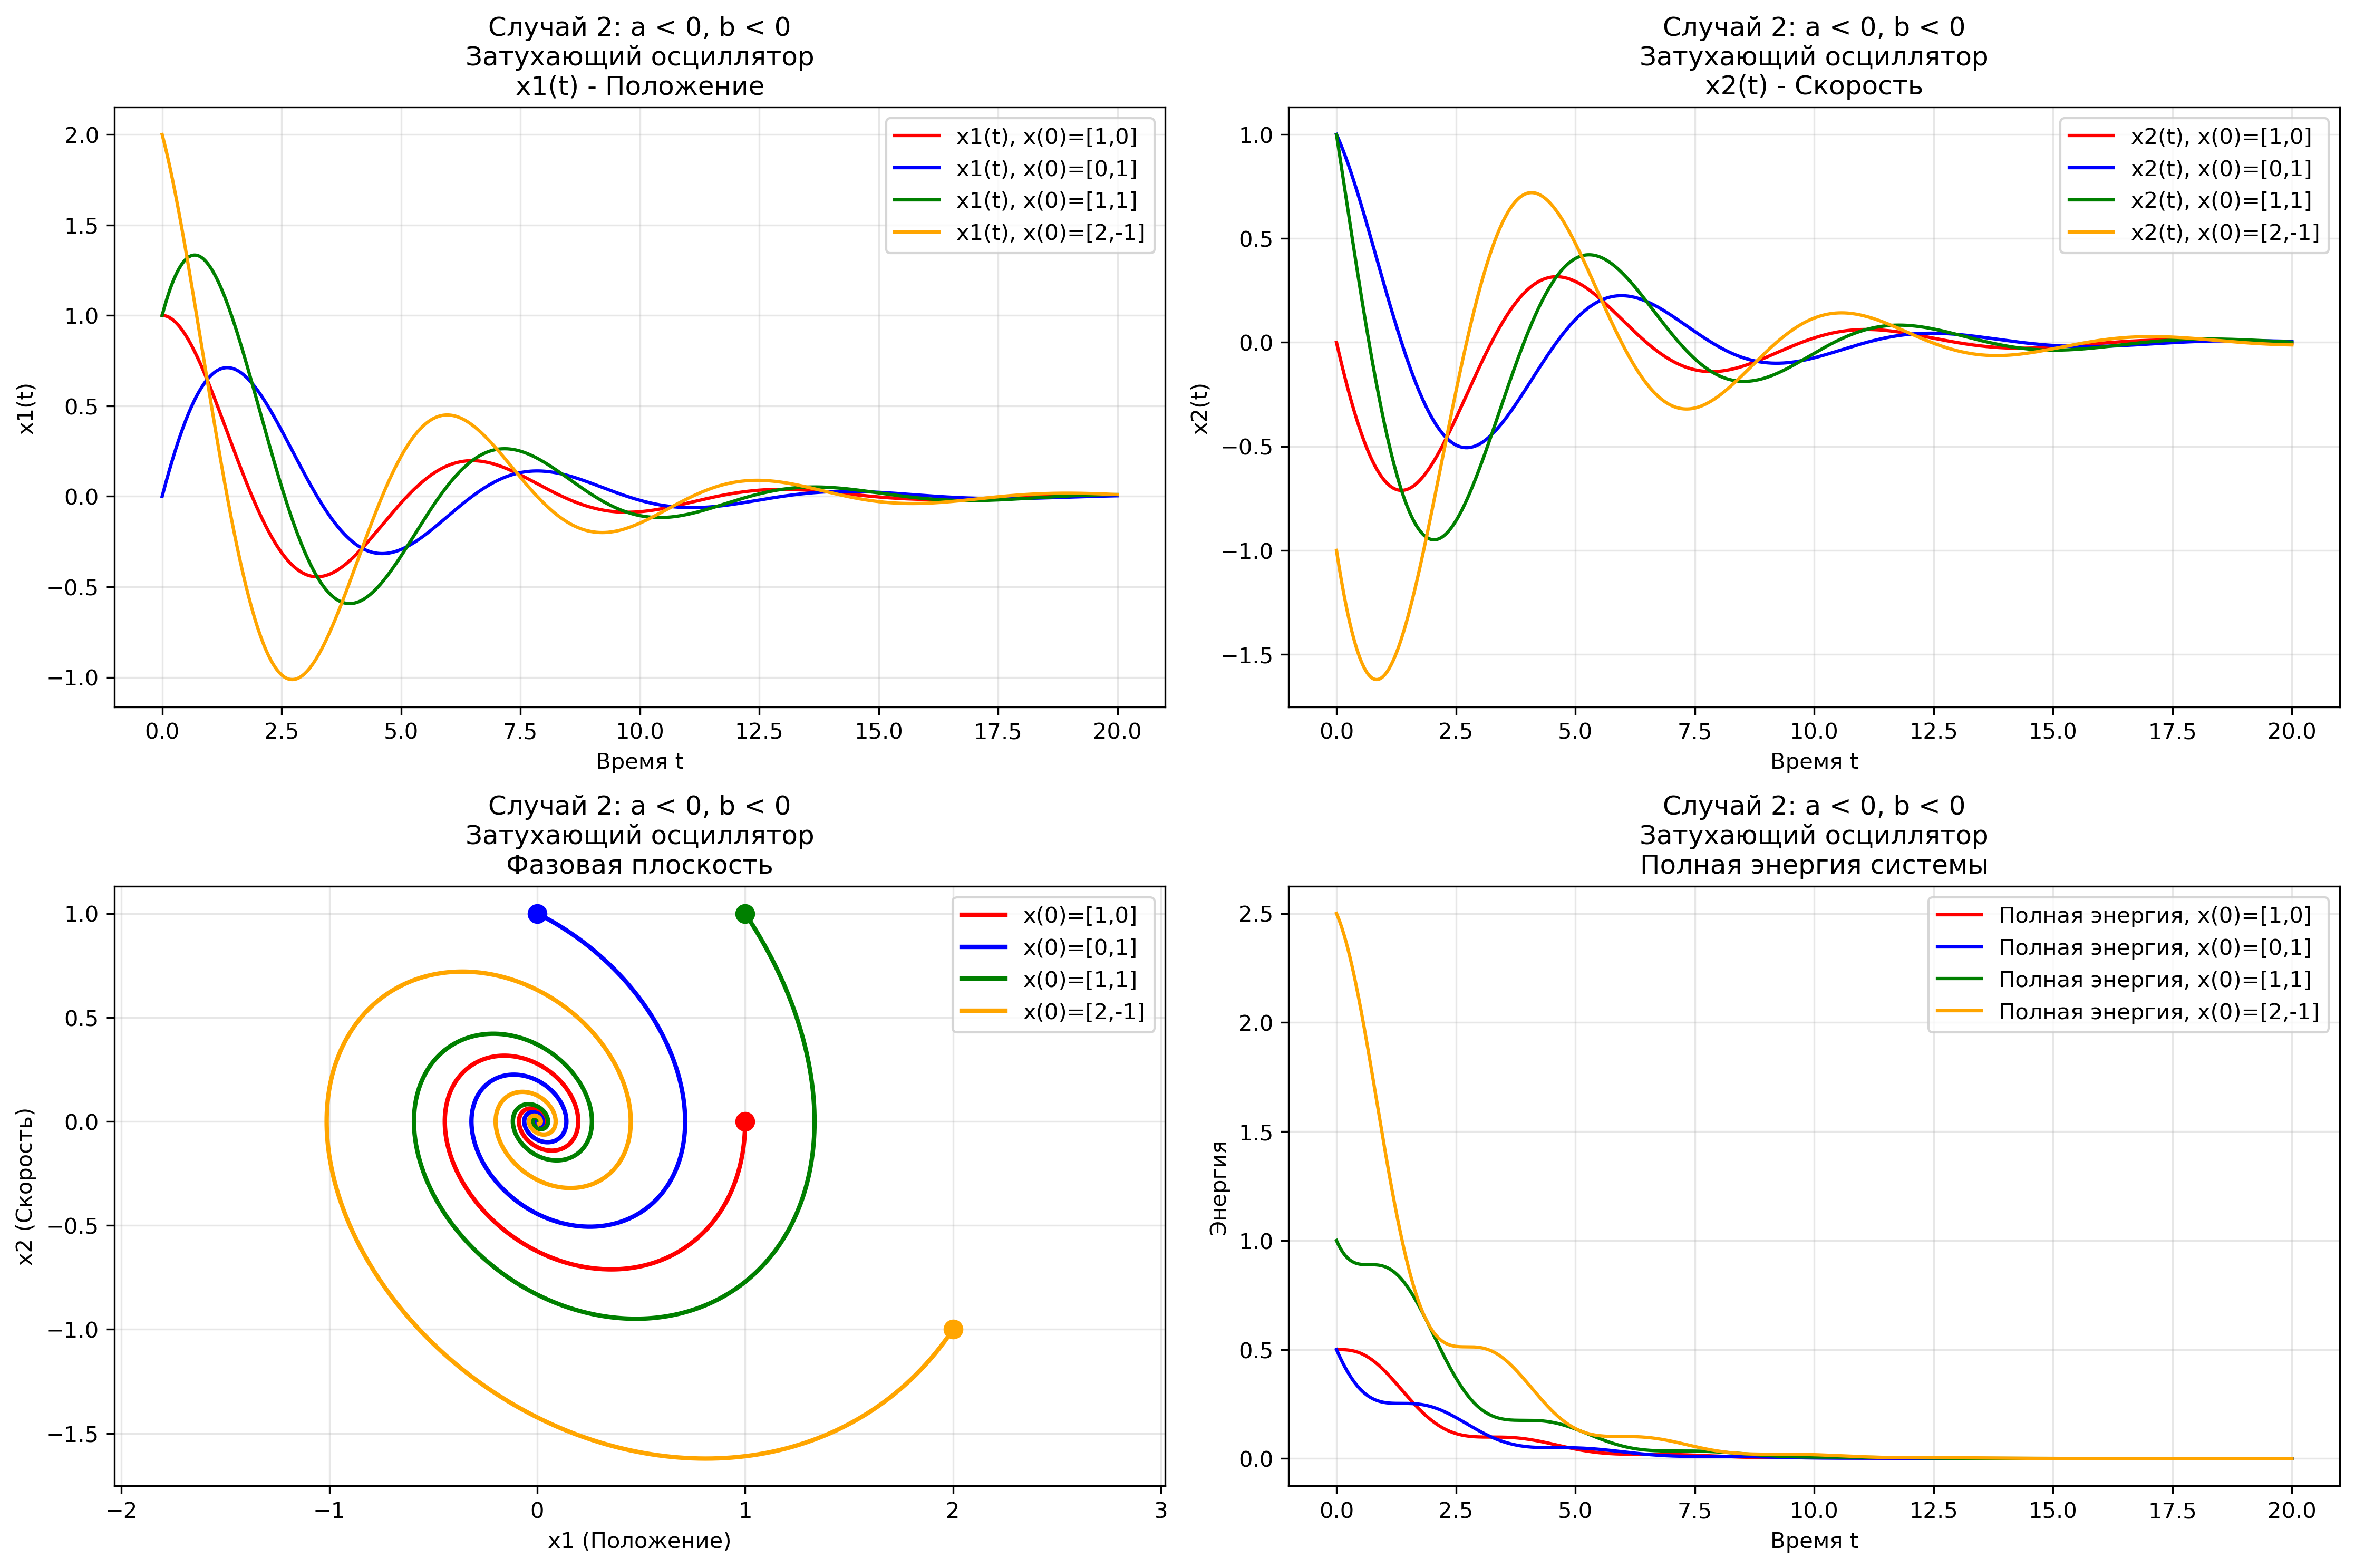
\includegraphics[width=0.9\textwidth]{images/task3/oscillator_case2_damped.png}
    \caption{Затухающий осциллятор: $a = -1$, $b = -0.5$}
\end{figure}

\textbf{Анализ:}
\begin{itemize}
    \item Собственные числа: $\lambda = -0.25 \pm 0.968i$ (отрицательные вещественные части)
    \item Тип устойчивости: Асимптотически устойчива
    \item Характер движения: Затухающие колебания
    \item Энергия системы уменьшается со временем
\end{itemize}

\subsection*{Случай 3: $a > 0$, $b = 0$ (Неустойчивый осциллятор)}

\textbf{Физическая интерпретация:} Неустойчивый осциллятор (перевернутый маятник)

\begin{itemize}
    \item $x_1$ - угол отклонения от неустойчивого равновесия
    \item $x_2$ - угловая скорость
    \item $a > 0$ - коэффициент неустойчивости (положительный для отталкивающей силы)
    \item $b = 0$ - отсутствие трения
\end{itemize}

\begin{figure}[H]
    \centering
    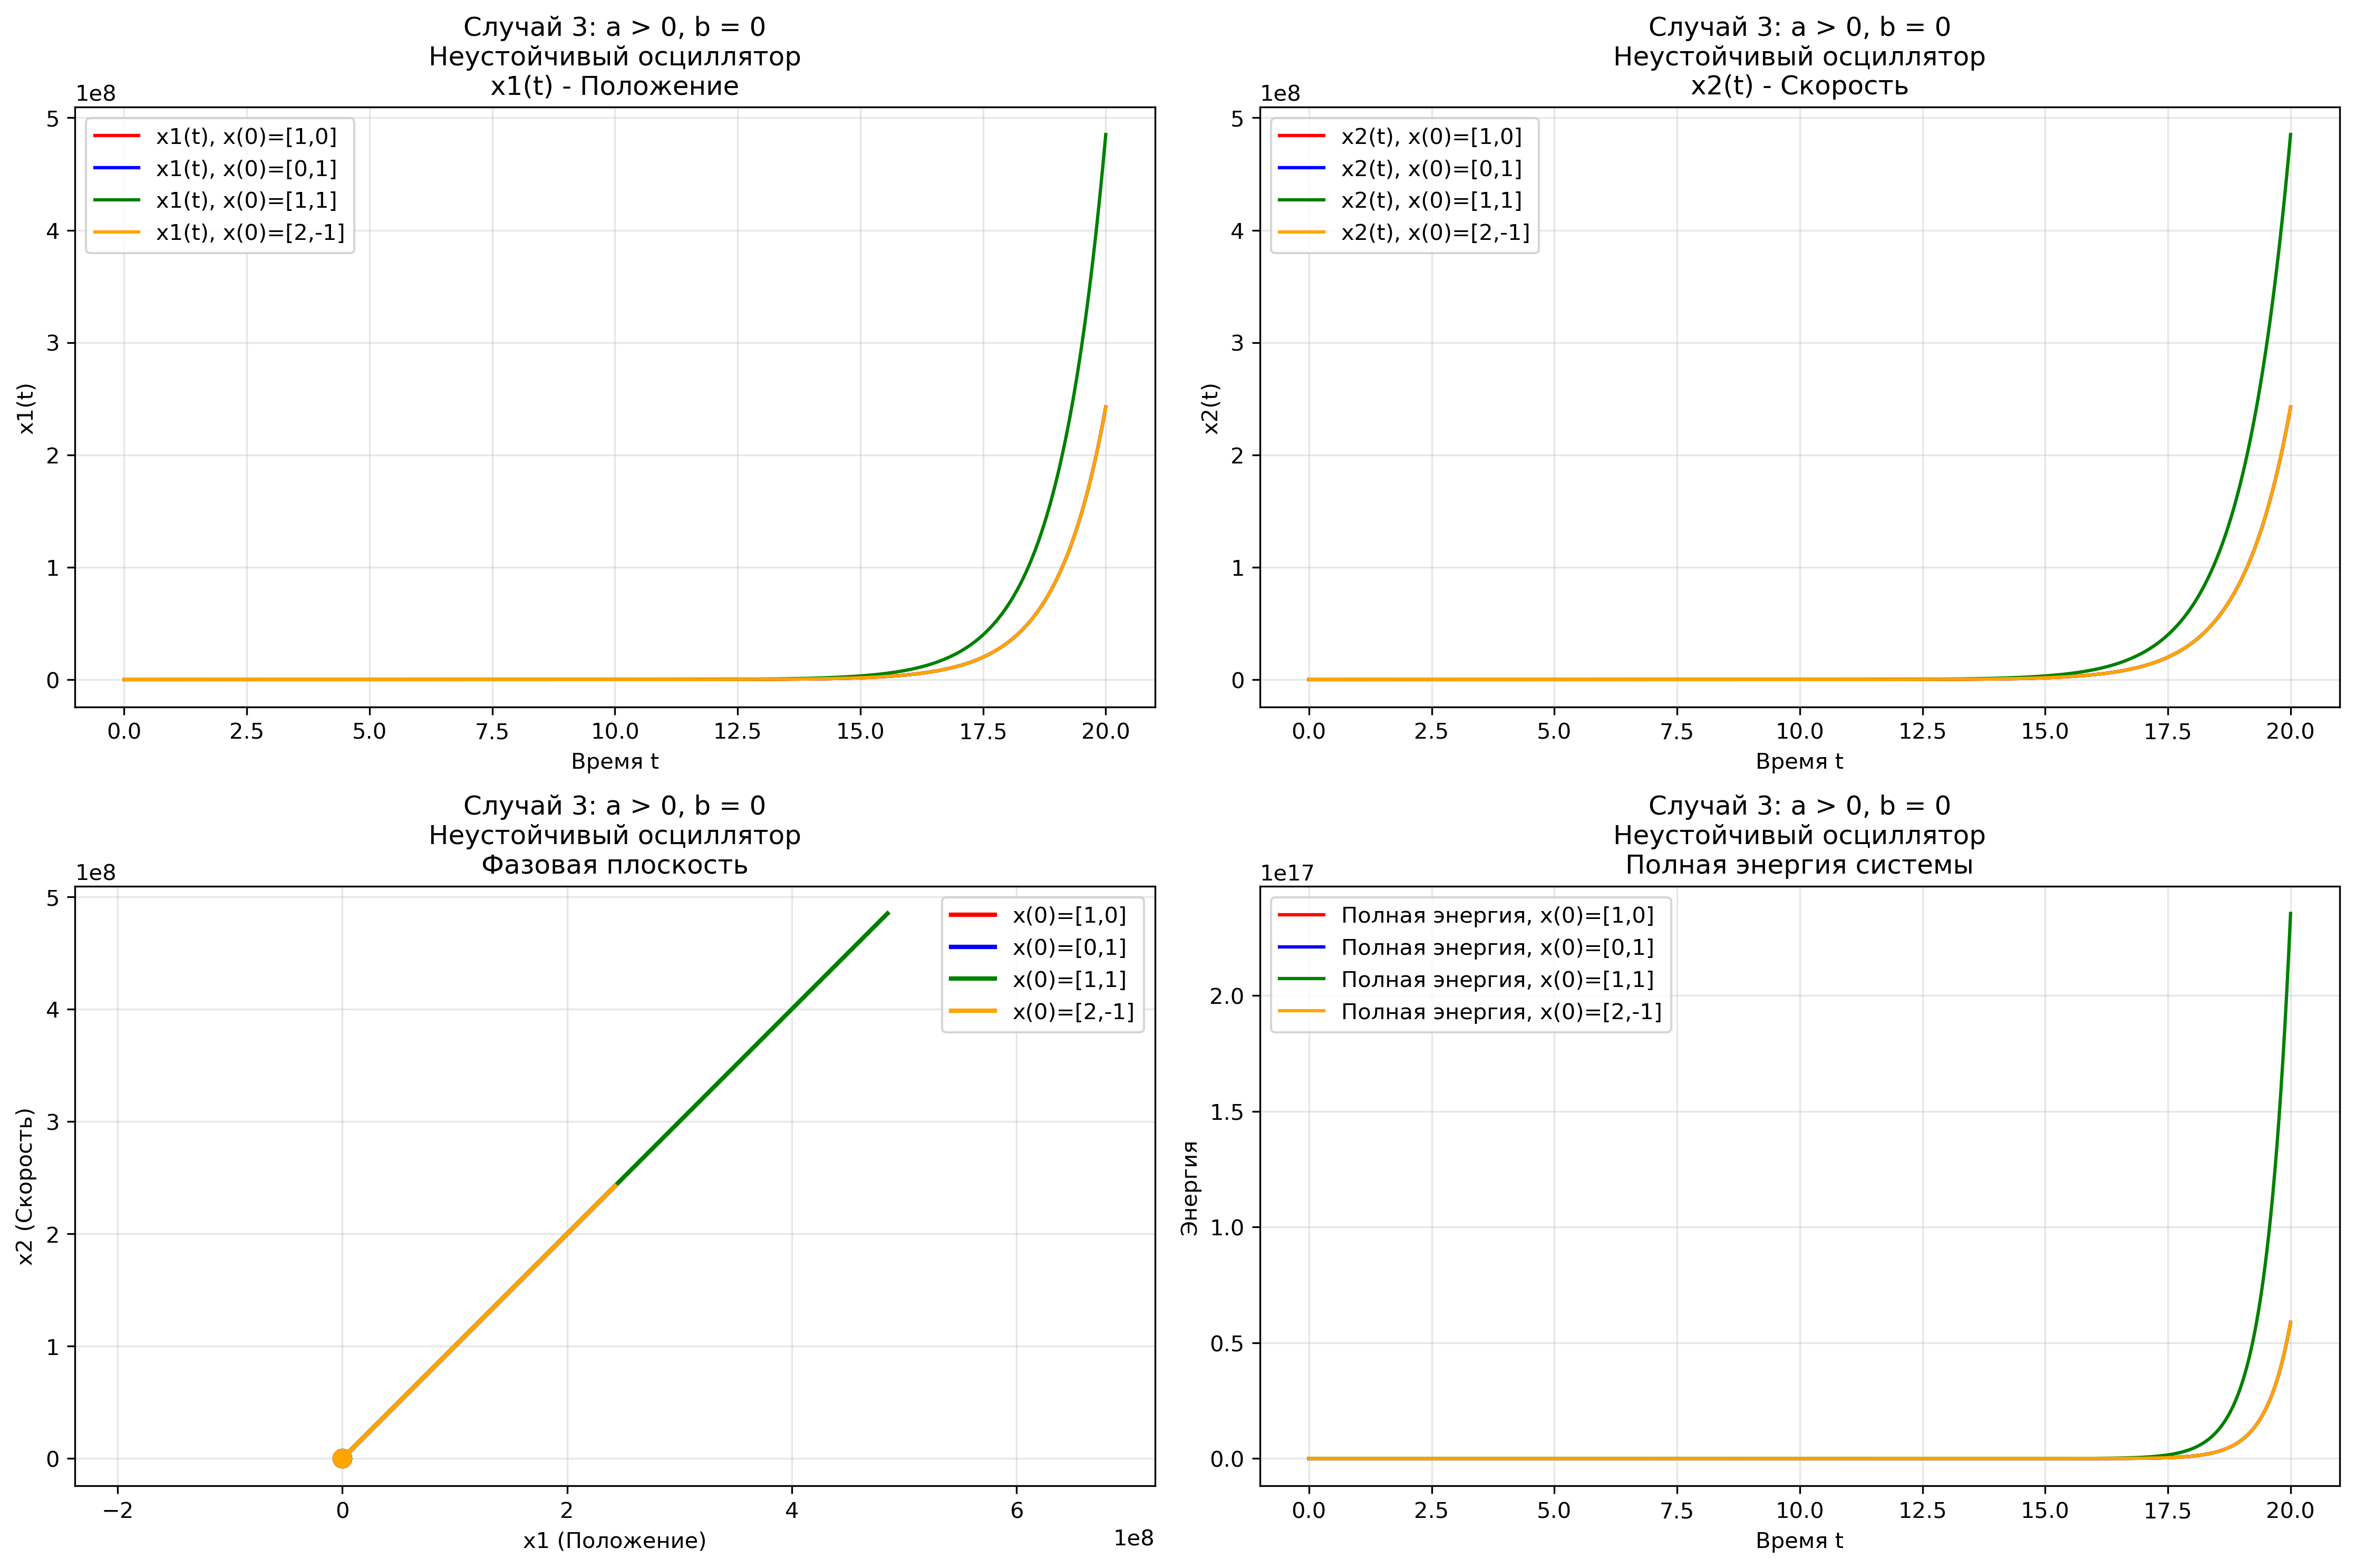
\includegraphics[width=0.9\textwidth]{images/task3/oscillator_case3_unstable.png}
    \caption{Неустойчивый осциллятор: $a = 1$, $b = 0$}
\end{figure}

\textbf{Анализ:}
\begin{itemize}
    \item Собственные числа: $\lambda = \pm 1$ (одно положительное, одно отрицательное)
    \item Тип устойчивости: Неустойчива
    \item Характер движения: Экспоненциальный рост
    \item Энергия системы растет со временем
\end{itemize}

\subsection*{Случай 4: $a > 0$, $b < 0$ (Неустойчивый осциллятор с затуханием)}

\textbf{Физическая интерпретация:} Неустойчивый осциллятор с затуханием

\begin{itemize}
    \item $x_1$ - отклонение от неустойчивого равновесия
    \item $x_2$ - скорость
    \item $a > 0$ - коэффициент неустойчивости
    \item $b < 0$ - коэффициент трения (может стабилизировать систему)
\end{itemize}

\begin{figure}[H]
    \centering
    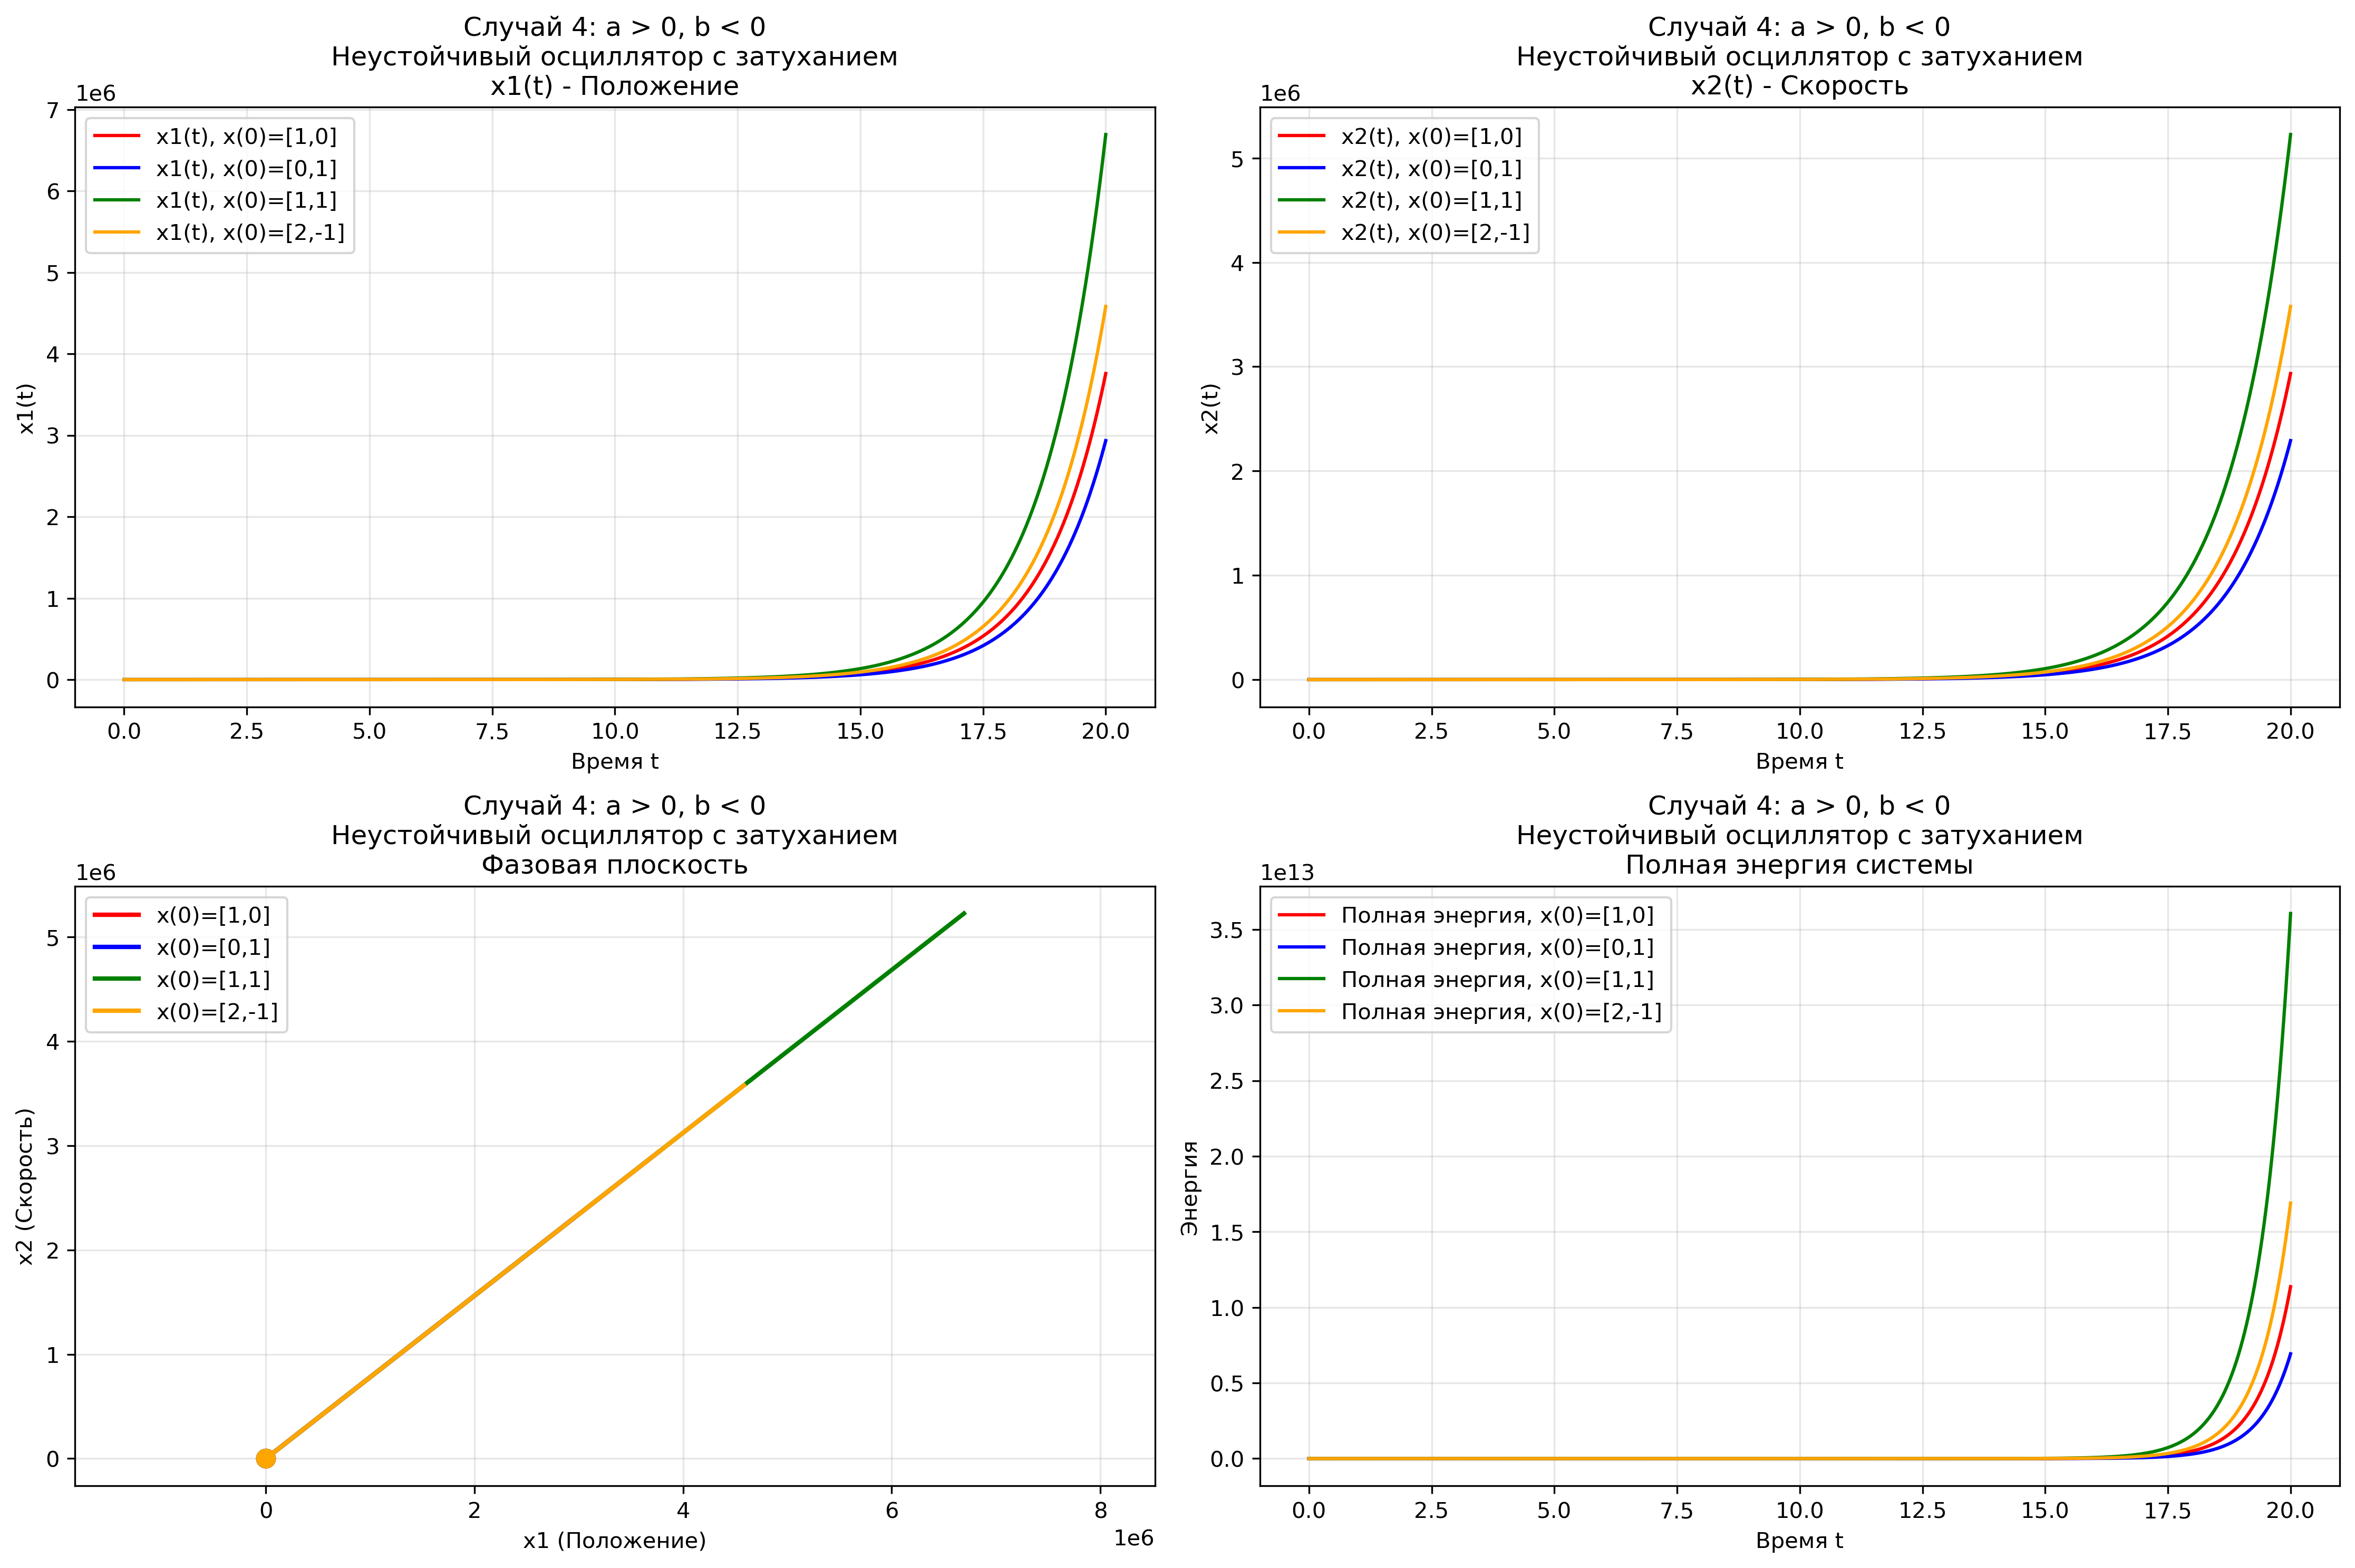
\includegraphics[width=0.9\textwidth]{images/task3/oscillator_case4_unstable_damped.png}
    \caption{Неустойчивый осциллятор с затуханием: $a = 1$, $b = -0.5$}
\end{figure}

\textbf{Анализ:}
\begin{itemize}
    \item Собственные числа: $\lambda = 0.781$, $\lambda = -1.281$ (одно положительное, одно отрицательное)
    \item Тип устойчивости: Неустойчива
    \item Характер движения: Экспоненциальный рост с затуханием по одной компоненте
    \item Трение не может полностью стабилизировать неустойчивую систему
\end{itemize}

\subsection*{Сравнительный анализ}

\begin{figure}[H]
    \centering
    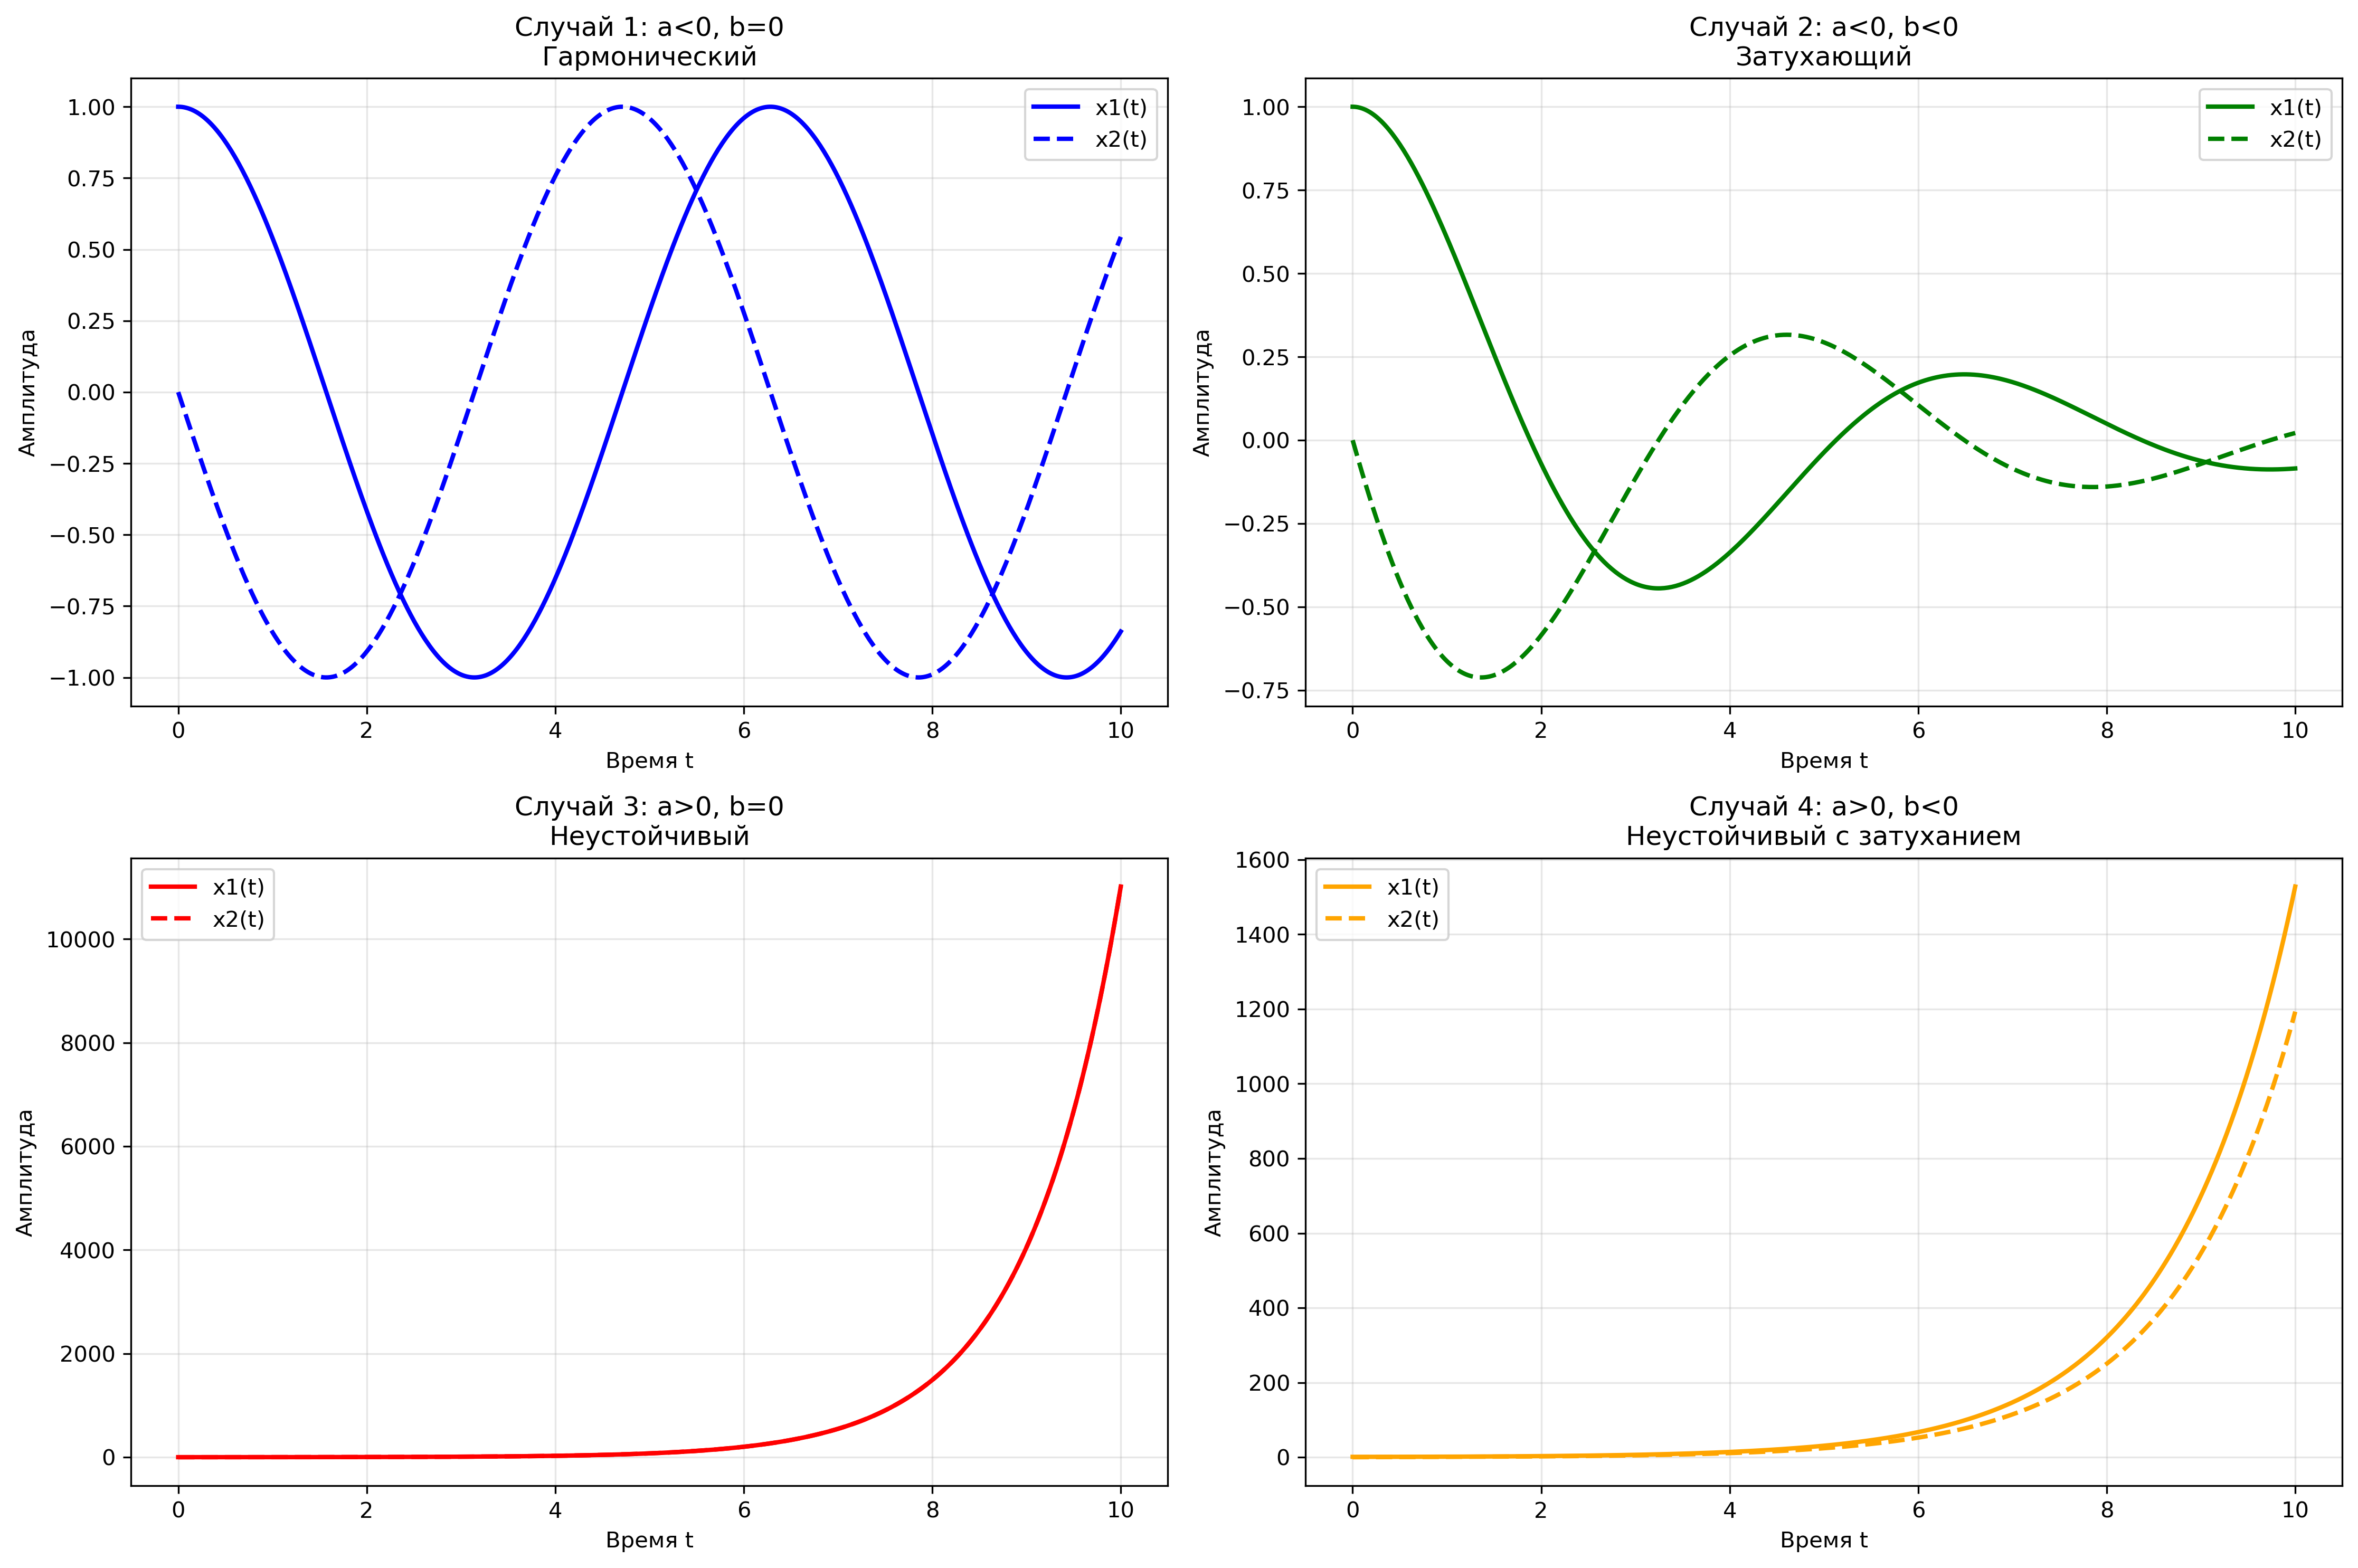
\includegraphics[width=0.9\textwidth]{images/task3/oscillator_comparison.png}
    \caption{Сравнение всех четырех случаев осциллятора}
\end{figure}

\textbf{Выводы:}
\begin{itemize}
    \item Параметр $a$ определяет тип равновесия: $a < 0$ - устойчивое, $a > 0$ - неустойчивое
    \item Параметр $b$ определяет наличие трения: $b < 0$ - затухание, $b = 0$ - отсутствие трения
    \item Комбинация параметров определяет характер движения системы
    \item Энергетический анализ подтверждает качественные выводы об устойчивости
\end{itemize}

\section*{Заключение}

В ходе выполнения лабораторной работы были изучены различные аспекты линейных динамических систем второго порядка.

\textbf{Основные результаты:}

\subsection*{Задание 1. Непрерывные системы}

\begin{itemize}
    \item Созданы шесть различных непрерывных систем с заданными свойствами устойчивости
    \item Исследовано влияние собственных чисел и собственных векторов на поведение системы
    \item Показано, что характер собственных чисел определяет тип устойчивости системы
    \item Демонстрированы различные типы траекторий: затухающие, растущие, периодические
\end{itemize}

\subsection*{Задание 2. Дискретные системы}

\begin{itemize}
    \item Созданы системы с заданными собственными числами
    \item Исследовано влияние модуля собственных чисел на устойчивость дискретных систем
    \item Показано, что $|\lambda| < 1$ обеспечивает асимптотическую устойчивость
    \item Демонстрировано влияние масштабирования на поведение системы
\end{itemize}

\subsection*{Задание 3. Осциллятор}

\begin{itemize}
    \item Проанализированы четыре различных случая осциллятора
    \item Дана физическая интерпретация параметров $a$ и $b$
    \item Показана связь между параметрами и типом устойчивости
    \item Проведен энергетический анализ системы
\end{itemize}

\textbf{Полученные навыки:}
\begin{itemize}
    \item Практическое применение теории собственных чисел для анализа устойчивости
    \item Создание и анализ динамических систем с заданными свойствами
    \item Моделирование и визуализация траекторий динамических систем
    \item Физическая интерпретация математических моделей
\end{itemize}

\textbf{Теоретическая значимость:} Изучены фундаментальные принципы теории динамических систем и их практическое применение.

\textbf{Практическая значимость:} Полученные навыки могут быть применены в различных областях: механика, электротехника, биология, экономика и других областях, где используются динамические системы.
